\documentclass{article}
\usepackage[utf8]{inputenc}
\usepackage{graphicx}
%\usepackage[latin1]{inputenc}
\usepackage[french]{babel}
\usepackage[T1]{fontenc}
\usepackage[top=2cm, bottom=2cm, left=1.5cm, right=1.5cm]{geometry}
\usepackage{enumitem}
\usepackage{floatrow}
\usepackage{subcaption}
\usepackage{subfiles}
\usepackage{titlesec}
\usepackage[table,xcdraw]{xcolor}
\usepackage{booktabs}
\usepackage{pdfpages}
\usepackage{afterpage}
\usepackage{pifont}
\usepackage{systeme}
\usepackage{array}
\usepackage{tabto}




\title{PPII S6 - Rapport}
\author{Armand Londeix, Patrick O'Brien, Lucas Rioux, Serge Téhé}
\date{Mars 2022 - Juin 2022}
\begin{document}

\begin{figure}
    \centering
    
\includegraphics[scale=0.15]{figures/logo_TNCY.png}
\end{figure}
\maketitle
\begin{center}
\large{Promotion 2024}
\end{center}

\noindent\makebox[\linewidth]{\rule{\paperwidth}{2pt}}
\bigbreak
\bigbreak
\bigbreak
\bigbreak

\begin{center}
\begin{Large}
\Huge\textsc{\textbf{PPII S6 : JEU WORDLE}}
\end{Large}
\end{center}
\bigbreak
\bigbreak
\bigbreak
\bigbreak
\noindent\makebox[\linewidth]{\rule{\paperwidth}{2pt}}

\bigbreak
\bigbreak
\begin{figure}[h!]
    \centering
    \includegraphics[scale=0.2]{figures/UnivLorraineCollégium.png}
\end{figure}

\begin{center}
\begin{Large}
Responsable du projet : Olivier Festor
                         

\end{Large}
\end{center}

\bigbreak
\bigbreak
\bigbreak
\bigbreak
\begin{center}
\large{28 mai 2022}
\end{center}

\newpage
\bigbreak
\bigbreak
\bigbreak
\bigbreak

\renewcommand{\contentsname}{Sommaire}
\tableofcontents{}
\newpage

\maketitle


\section{Introduction}
\subsection{Objectif du projet}

\tabto{1cm}L'objectif de ce projet est de recréer le jeu Wordle du New York Times tout en y ajoutant de nouvelles fonctionnalités, telles qu'un historique des parties, des succès à débloquer, des statistiques de jeu ainsi que la possibilité de paramétrer les parties en choisissant à la fois la longueur du mot à trouver et le nombre de tentatives autorisées. Cette application sera implémentée selon une architecture trois-tiers (Python, base de données et interface Web).\\

\tabto{1cm}En parallèle de cette application, un solveur sera développé en C. Ce solveur aura évidemment pour objectif de résoudre le jeu le plus rapidement et efficacement possible. Il sera interactif : le joueur pourra y soumettre les mots qu'il a choisis au cours d'une partie et le solveur renverra alors le meilleur mot possible en fonction de ces informations. Le développement de ce solveur s'appuie notamment sur la théorie de l'information. 

%La fonctionnalité la plus importante était un solveur qui peut essentiellement jouer le jeu Wordle en cherchant un mot choissi par l'utilisateur, tandis que l'utilisateur donne des indices de la manière normale du jeu. Les autres nouveautés consistaient en une page de réalisations et en divers modes de jeu. Afin de sauvegarder les différents succès et les détails de chaque partie, le joueur est obligé de se connecter, mais cela n'est pas nécessaire si l'utilisateur souhaite jouer à un jeu directement comme le jeu orignal. L'application a été réalisé sur un architecture de Python/Web/Base de données et le solveur a été code en C.

\subsection{Règles du jeu de WORDLE}

\begin{figure}[h!]
\centering
\begin{subfigure}{.5\textwidth}
  \centering
  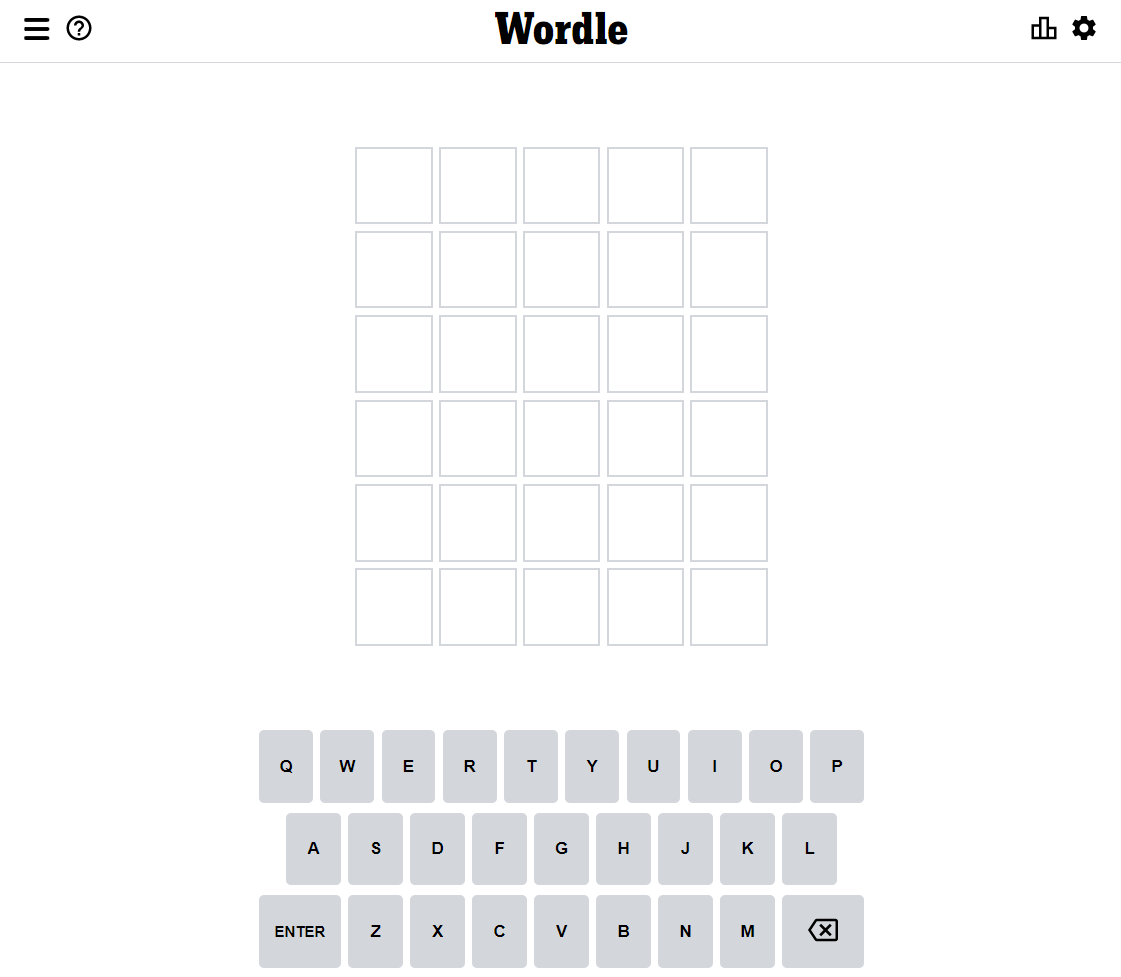
\includegraphics[width=.8\linewidth]{figures/wordle.jpeg}
\end{subfigure}%
\begin{subfigure}{.5\textwidth}
  \centering
  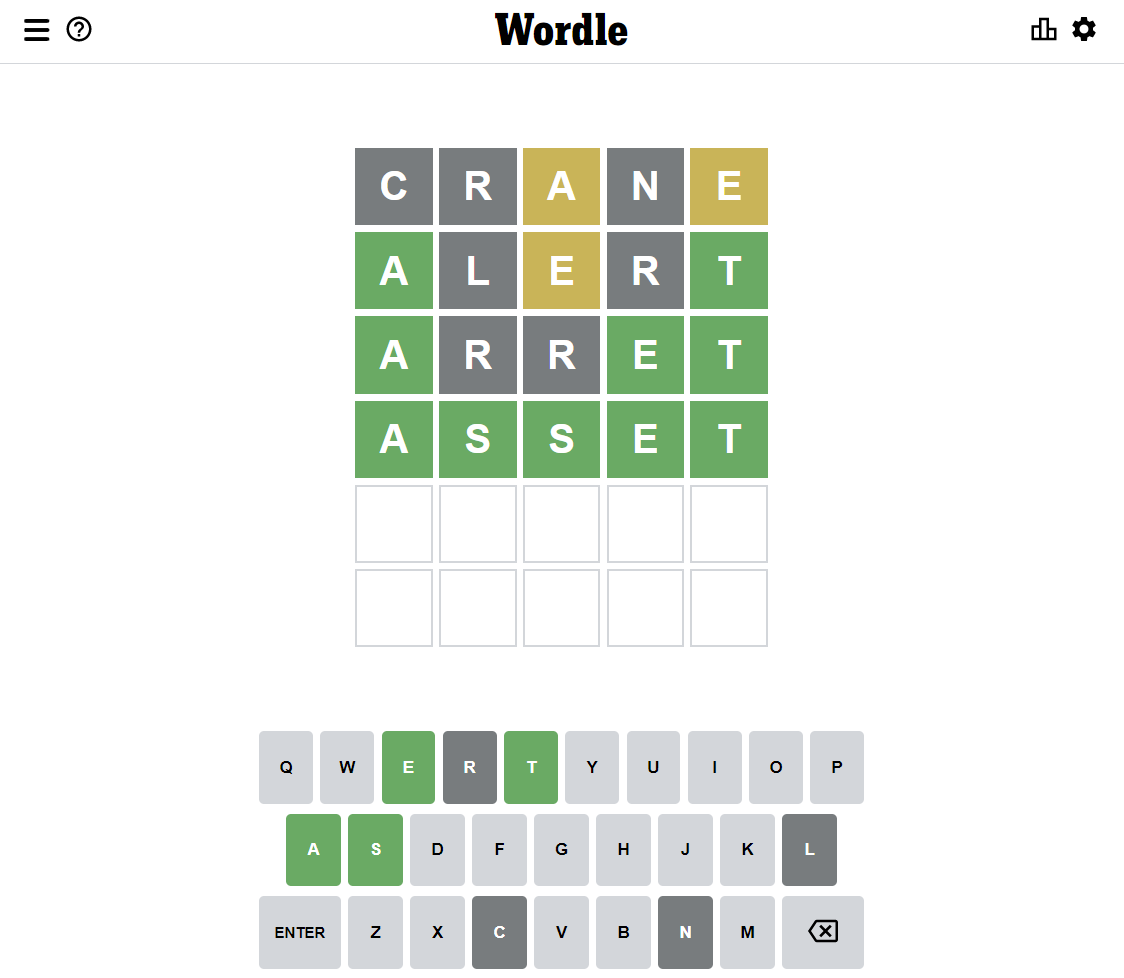
\includegraphics[width=.8\linewidth]{figures/wordle_asset.jpeg}
\end{subfigure}
\caption{Wordle - The New York Times}
\label{fig:test}
\end{figure}

\tabto{1cm}Le joueur a  jusqu'à six tentatives pour deviner un mot de cinq lettres. Après chaque tentative, le jeu montre les lettres qui correspondent à la réponse ; si l'une des 5 lettres devinées apparaît dans la réponse et a également été placée au bon endroit, elle est mise en évidence en vert. Si la lettre apparaît dans la réponse mais n'a pas été placée au bon endroit, elle est sur-lignée en jaune. Si la lettre est complètement fausse, elle devient grise. \\ \\
\tabto{1cm}En bas de la page, le joueur peut voir un clavier QWERTY avec les lettres utilisées sur-lignées en vert, jaune ou gris en fonction des essais précédents. Le joueur peut seulement essayer des mots existants dans le dictionnaire de mots possibles, c'est-à-dire que le joueur ne peut pas rentrer des mots aléatoires ou inexistants dans le but d'obtenir des indices plus rapidement (exemple : AEIOU en français). S’il essaye un mot qui n’est pas dans le dictionnaire, le jeu ne l’accepte pas et le joueur doit en proposer un autre.

\tabto{1cm}



\newpage
\section{Implémentation de WORDLE}

\subsection{La base de données}
Notre base de données est constituée de 4 tables:
\vspace*{0.5cm}
\begin{itemize}
    \item Une table \texttt{Utilisateur} stockant les informations des joueurs. Ses colonnes sont : \texttt{idUser} qui est l’identifiant du joueur de type entier, son nom d'utilisateur \texttt{pseudo} de type str, un mot de passe \texttt{motDePasse} de type str et un sel  \texttt{salt} pour la sécurisation du compte utilisateur. La chaîne de caractères stockée dans la colonne \texttt{motDePasse} sera le haché de la concaténation du mot de passe et du salt.
     \vspace*{0.2cm}
    
    \item Une table \texttt{Partie} qui stocke les données des parties jouées de chaque joueur connecté. Ses colonnes sont : \texttt{idPartie} qui représente l’identifiant d’une partie de type int, \texttt{idUser} qui est une clé étrangère référençant l'identifiant de l'utilisateur, les points d'expérience \texttt{pts\_experience} de type int qui représentent les points gagnés lors d’une partie, le mot à deviner \texttt{motSecret} associé à la partie de type str, le nombre d'essais utilisés par le joueur pour trouver le mot secret \texttt{nb\_coups} de type int, le nombre d’essais maximum de la partie \texttt{nb\_essais\_maximum} de type int, la longueur des mots associée au mot de la partie \texttt{longueur\_mot} de type int et le mode de jeu défini par le joueur \texttt{modejeu} (mode sans fin ou mode classique).
     \vspace*{0.2cm}
    
    \item Une table \texttt{AchievementDesc} qui stocke les descriptions des achievements. Ses colonnes sont : \texttt{idSucces} qui est l’identifiant de l’achievement et \texttt{description} la description associée : gagner une partie en 3 coups ou moins, gagner 10 parties, etc\dots{}
     \vspace*{0.2cm}
    
    \item Une table \texttt{Achievements} qui relie les tables \texttt{AchievementDesc} et \texttt{Partie} dont les colonnes sont : \texttt{idPartie}, clé étrangère qui référence l'identifiant d'une partie et \texttt{idSucces}, clé étrangère référençant l'identifiant d'un achievement. Ces 2 clés forment la clé primaire de la table \texttt{Achievements}.
\end{itemize}

Notre base de données est en 3ème forme normale.

\begin{figure}[h!]
    \centering
    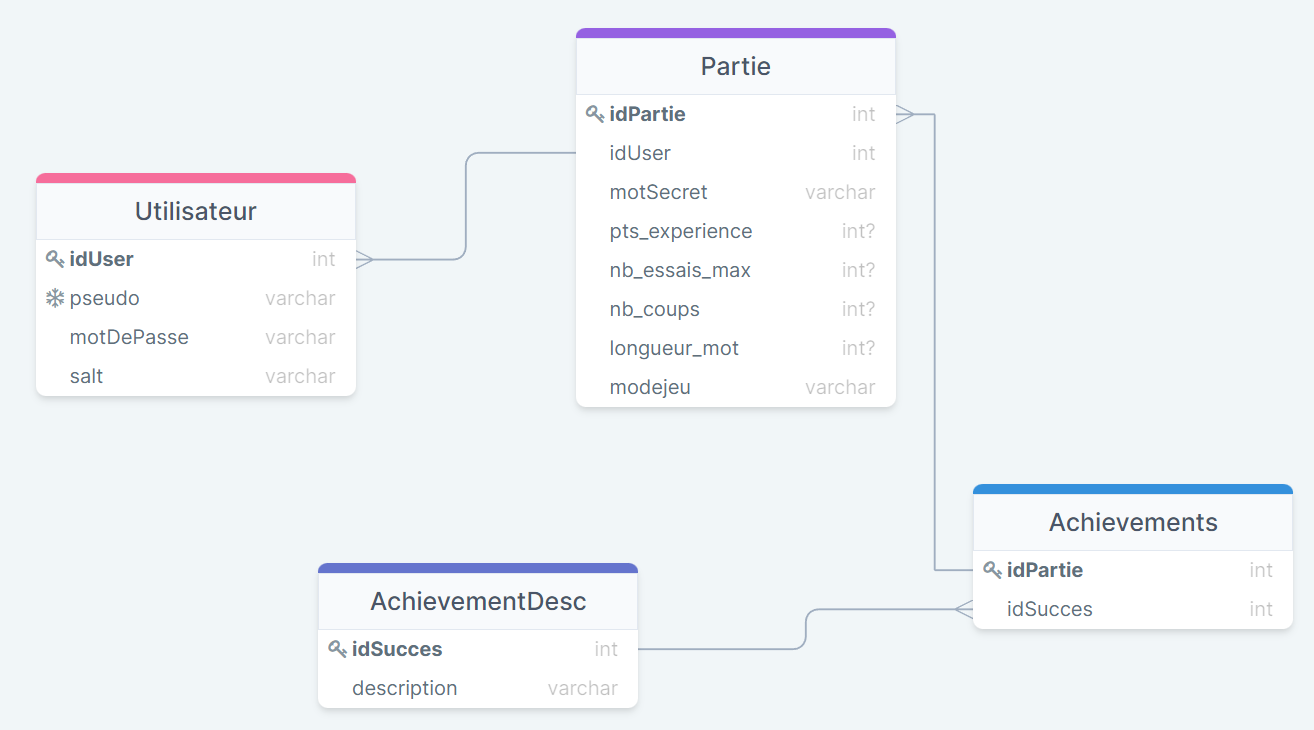
\includegraphics[width=16cm]{figures/bddfinale.PNG}
    \caption{Schéma de la base de données de WORDLE}
\end{figure}

\begin{figure}[h!]
    \centering
    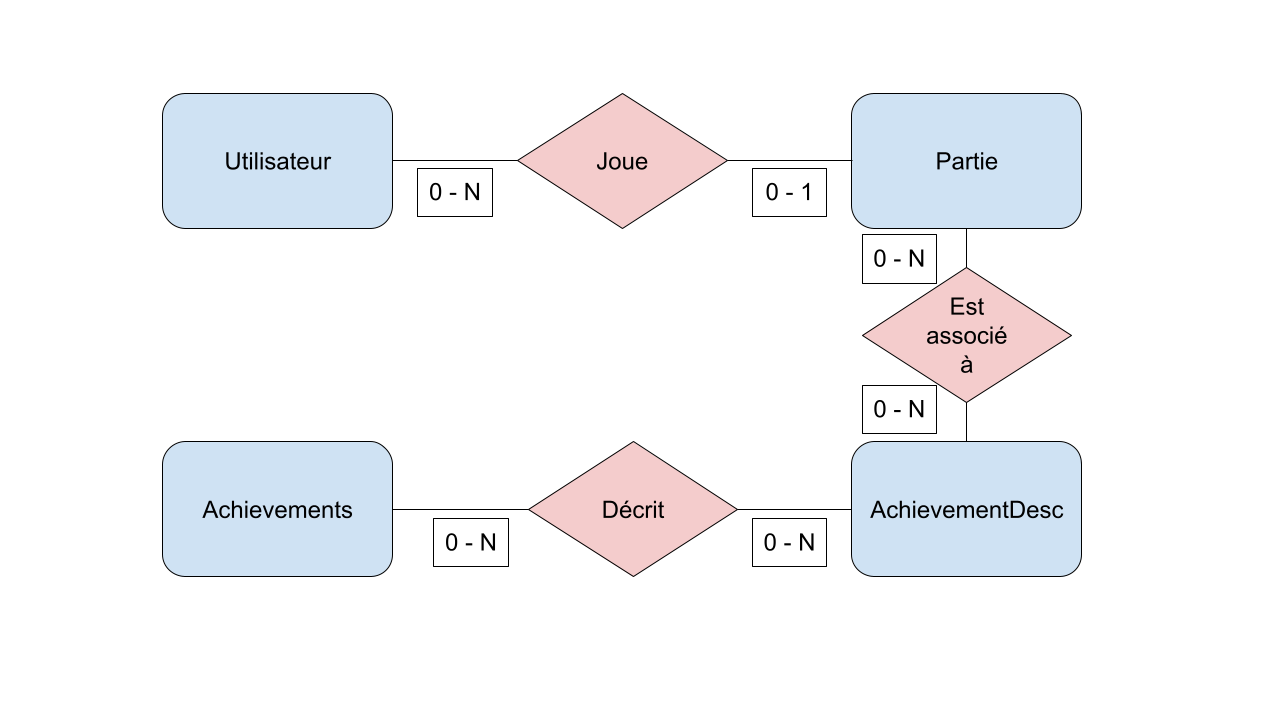
\includegraphics[width=16cm]{figures/modele_entite_association.png}
    \caption{Modèle entité-association de la base de données}
\end{figure}

\newpage 
\subsection{L'interface Web}
\tabto{1cm}L'application a été développée en langage Python avec le framework Flask, permettant ainsi de créer et gérer des pages HTML dynamiques. Le fichier contrôleur, \emph{app.py}, permet de rediriger l'utilisateur sur les bonnes routes en fonction de la position sur le site et de la validité de ses réponses aux différents formulaires. Ce fichier gère également les requêtes SQL avec la base de données \emph{database.db}, notamment \texttt{INSERT INTO} et \texttt{SELECT}. Le jeu WORDLE a, quant à lui, été implémenté en JavaScript.\\

Ce tableau récapitule le fichier correspondant à chacune des différentes routes :

\begin{center}
\begin{tabular}{|c|c|c|}
    \hline
    \textbf{Route} & \textbf{Page HTML associée} & \textbf{Fonctionnalités} \\
    \hline
    \emph{/} & \emph{index.html} & Jeu WORDLE \\
    \hline
    \emph{/register} & \emph{register.html} & Créer un compte \\
    \hline
    \emph{/login} & \emph{login.html} & Se connecter au jeu \\
    \hline
    \emph{/preference} & \emph{preference.html} & Modifier les paramètres du jeu \\
    \hline
    \emph{/profile} & \emph{profile.html} & Consulter son historique de jeu, ses succès et ses statistiques \\
    \hline
    \emph{/logout} & Aucune & Se déconnecter \\
    \hline
    \emph{/recup/<userinfo>} & Aucune & Récupérer les informations relatives à une partie depuis \emph{index.js} \\
    \hline
\end{tabular}
\end{center}

\vspace{0.5cm}

\tabto{1cm}Dans la suite de cette partie du rapport (\textbf{Interface Web}), on confondra route et page HTML associée pour les 5 premières routes du tableau.

\subsubsection*{Jouer à WORDLE}

\tabto{1cm}La page d'accueil du site est \emph{index.html}, sur la route \emph{/}. Sur cette page, le joueur peut directement faire une partie et modifier les paramètres de jeu (longueur du mot, nombre de tentatives) s'il souhaite en cliquant sur le bouton \textbf{Paramètres de jeu} qui le redirigera sur la route \emph{/preference}. Le joueur peut également choisir le mode de jeu de WORDLE : soit classique (le jeu de base), soit sans fin. Dans ce second mode, il faut deviner le plus de mots possibles d'affilée sans se tromper sans quoi le jeu s'arrêtera. \\

\tabto{1cm}À noter que ces paramètres sont stockés dans la variable globale \emph{session}, ce qui permet même à un joueur non connecté de changer ces paramètres à sa guise. De plus, au lancement du jeu, la fonction \emph{before\_first\_request()} s'exécute et déconnecte automatiquement un joueur potentiellement connecté et réinitialise les paramètres de jeu dans le but d'éviter des bugs.\\

\tabto{1cm}Laisser la possibilité au joueur de créer un compte ou non lui permet de jouer directement et ainsi rend le jeu plus attractif : des joueurs pourraient être repoussés à l'idée d'être forcés de créer un compte. C'est pourquoi il n'est pas obligatoire de créer un compte pour jouer. Cependant, les parties et leurs informations jouées par un joueur non connecté ne sont pas enregistrées, même si les seules informations demandées sont un pseudonyme et un mot de passe.

\subsubsection*{S'inscrire, se connecter, se déconnecter}

\tabto{1cm}Pour s'inscrire, il suffit de cliquer sur le bouton \textbf{S'inscrire} en haut à droite de la page d'accueil. Dans ce cas, le joueur est redirigé sur la route \emph{/register} et on lui demande un pseudonyme et un mot de passe, qu'il doit ensuite confirmer. Ces deux informations doivent faire entre 8 et 20 caractères, dans le but de rendre l'application un peu plus sécurisée. Il est impossible de choisir un pseudonyme déjà pris par un autre joueur, et les deux mots de passe renseignés doivent être évidemment identiques. \\

\tabto{1cm}En cas d'échec d'inscription pour les raisons évoquées ci-dessus, le joueur reste sur la même route et les champs du formulaire sont effacés, sinon les informations du joueur sont ajoutées à la table \texttt{Utilisateur} de la base de données, puis le joueur est redirigé sur la route \emph{/login}. Pour plus de sécurité, le mot de passe est concaténé avec un salt de longueur 12 avant d'être haché avec la fonction \emph{SHA256}, puis seulement enregistré.\\

\tabto{1cm}Sur la page de connexion, il suffit de rentrer ses informations d'authentification pour se connecter. Une fois connecté, le psuedonyme du joueur s'affiche en haut à droite avec la mention "En ligne" (un joueur non connecté verrait la mention "Hors ligne" s'afficher). De plus, son id de joueur (selon la base de données) et son pseudonyme sont ajoutés à session, ce qui permet de savoir que ce joueur est connecté.\\

\tabto{1cm}Pour se déconnecter, il suffit de cliquer sur le bouton \textbf{Se déconnecter} une fois connecté. Le joueur est alors redirigé sur la route \emph{/logout}, où \emph{session} est vidé de l'id du joueur et de son pseudonyme, puis le joueur est redirigé vers la route \emph{/}.

\subsubsection*{Profil d'un joueur}

\tabto{1cm}Un joueur \textbf{connecté} à automatiquement accès à son profil via le bouton \textbf{Profil}, qui le redirige alors sur la route \emph{/profile} (un joueur non connecté n'a pas accès à cette fonctionnalité). La page \emph{profile.html} recense l'historique de ces parties, les succès débloqués, les statistiques de jeu et l'expérience du joueur. Dès que le joueur se rend sur cette route, toutes ces données sont actualisées grâce aux fonctions \emph{getHistorique()}, \emph{getStatistiques()}, \emph{achQuests()} et \emph{niveau()} respectivement. Aucune de ces fonctions ne prend l'ID du joueur en argument puisque ce dernier est stocké dans \emph{session} avec la clé \emph{idUser}.

\subsubsection*{Profil d'un joueur - [1] Historique}

\tabto{0cm}Pour chaque partie jouée, on enregistre :
\begin{itemize}
    \item le mot à deviner;
    \item sa longueur;
    \item le nombre de tentatives autorisées;
    \item le nombre de tentatives utilisées pour deviner le mot (-1 en cas de défaite);
    \item l'expérience gagnée à l'issue de la partie (0 en cas de défaite);
    \item le mode de jeu ("Classique" ou "Sans fin").
\end{itemize}

Ces informations sont récupérées depuis le fichier \emph{dash.js} puis envoyées à \emph{app.py} via la route \emph{/recup/<userinfo>} avec une requête XML HTTP, dans un fichier \emph{.json}. Ces données sont ensuite enregistrées dans la table \texttt{Partie}.\\

\tabto{1cm}L'historique est récupéré en exécutant la fonction \emph{getHistorique()}, puis est ensuite affiché de la partie la plus récente à la plus ancienne. Pour chacune d'entre elles, la couleur informe le joueur de sa victoire (vert) ou de sa défaite (rouge). Les informations enregistrées dans \texttt{Partie} sont également affichées pour plus de détails sur chaque partie. L'équipe projet a décidé de n'implémenter que le minimum demandé concernant l'historique pour se concentrer sur d'autres fonctionnalités détaillées plus loin.

\subsubsection*{Profil d'un joueur - [2] Achievements (succès)}

\tabto{1cm}En jouant au jeu, le jouer peut débloquer des achievements en réalisant certaines tâches, comme jouer ou gagner un certain nombre de parties ou en gagnant une partie en 3 essais ou moins. Sur la page \emph{profile.html}, les achievements débloqués sont en vert tandis que ceux pas encore débloqués sont en violet. \\

\tabto{1cm}Dès que le joueur se rend sur la route \emph{/profile}, on exécute la fonction \emph{achQuests(idPartie)} qui récupère en premier lieu la liste des IDs des achievements déjà débloqués avec la fonction \emph{getAchsAlreadyUnlocked()}. Ensuite, pour chacun d'entre eux, on exécute une requête SQL puis on analyse son résultat, dans le but de savoir si on délivre tel achievement au joueur ou non. Si la condition d'obtention de l'achievement est vérifiée et qu'il n'est pas encore débloqué, on exécute la requête SQL \texttt{INSERT INTO Achievements VALUES (idPartie, idSucces)} pour donner l'achievement \texttt{idSucces} au joueur. idPartie est l'ID de la dernière partie jouée par le joueur : ainsi, on s'assure d'effectuer les requêtes SQL sur l'ensemble des parties jouées par le joueur connecté.

%Dès que un achievement est débloqué le I.D. de la partie et le I.D. de l'achievement sont enregistrés dans la table 'Achievements' de la base de données. Si le joueur veut regarder tous les achievements qu'il a débloqué il peut voir la page ''. Sur cette page on peut voir tous les achievements possible. L'achievement est sur-ligné en vert s'il est débloqué, sinon il reste rouge. En haut de la page on a un niveau et une barre d'expérience qui augmentent en fonction du nombre de parties que le joueur a joué, le nombre de lettres de la partie et le nombre d’essais de la partie nécessaires. Évidement, ce n’est que possible d’enregistrer un achievement si le joueur est connecté en débloquant l’achievement et ce n’est que possible de voir les achievements débloqués si le joueur est connecté.

\subsubsection*{Profil d'un joueur - [3] Statistiques}

\tabto{1cm}Sur la page \emph{profile.html}, on retrouve un tableau recensant les statistiques de jeu du joueur : moyenne du nombre de coups pour les parties gagnées, nombre de parties jouées et taux de victoires. Les statistiques sont d'abord présentées pour l'ensemble des parties jouées, puis détaillées selon le nombre de lettres. On retrouve aussi la plus grande série de victoires (le plus grand nombre de parties gagnées d'affilée), calculé avec la fonction \emph{getBestStreak()}.\\

\tabto{0cm}Ces informations sont récupérées grâce à la fonction \emph{getStatistiques()}, qui renvoie un tuple de longueur 6 contenant :
\begin{itemize}
    \item la moyenne du nombre de coups pour toutes les parties gagnées;
    \item une liste contenant la moyenne du nombre de coups pour les parties gagnées avec des mots de 4 à 12 lettres inclus;
    \item le nombre de parties jouées;
    \item une liste contenant le nombre de parties jouées avec des mots de 4 à 12 lettres inclus;
    \item le taux de victoires en \%;
    \item une liste contenant le taux de victoires en \% avec des mots de 4 à 12 lettres inclus.
\end{itemize}

%\tabto{1cm}Dans l'onglet profile se trouve une partie dédiée aux statistique qui se présente sous la forme d'un tableau possédant autant de ligne que de nombre de lettre à choisir plus une qui correspond aux statistiques globales. Pour chaque nombre de lettre et pour toutes les parties (les statistiques globales) le tableau nous donne le nombre de coups moyen, le nombre de parties jouées ainsi que le taux de victoire.

\subsubsection*{Profil d'un joueur - [4] Expérience}

\tabto{1cm}L'expérience représente le temps passé sur le jeu par le joueur, ainsi que sa capacité à bien jouer. Lorsqu'un joueur crée un compte, il est au niveau 1 et il peut monter jusqu'au niveau 100. Perdre une partie rapporte 0 point d'expérience. Pour chaque partie gagnée, le joueur gagne de l'expérience selon la formule suivante :

\begin{equation}
    expGagnee = (nbEssaisMax - nbEssaisUtilises) * 100 + longueurMot * 200 - nbEssaisMax * 20
\end{equation}

\tabto{0cm}avec :
\begin{itemize}
    \item nbEssaisMax : le nombre d'essais maximum autorisés pour cette partie;
    \item nbEssaisUtilises : le nombre d'essais utilisés par le joueur pour deviner le mot;
    \item longueurMot : la longueur du mot (en lettres).
\end{itemize}

\tabto{0cm}Pour calculer le nombre de points d'expérience nécessaires pour passer au niveau suivant, on utilise la formule :

\begin{equation}
    expNecessaire = \lfloor 1.05 * x^\frac{9}{4} \rfloor
\end{equation}

\tabto{0cm}où $x$ représente le niveau à atteindre (entre 2 et 100).

%Pour le jeu lui-même, nous voulions quelque chose de facile à utiliser mais avec quelques fonctionnalités supplémentaires. Tout comme le jeu WORDLE original, nous permettons à nos utilisateurs de démarrer un jeu directement à partir de la page d'accueil, mais afin de suivre les statistiques du jeu, il faut enregistrer ses coordonnées dans la base de données. Les règles du jeu sont, pour la plupart, comme celles du WORDLE original mais on peut changer les paramètres ; longueur de mot et nombre de tentatives. Si l'utilisateur décide de créer un compte, il aura accès à sa progression et à un score qui peut représenter son nombre moyen de tentatives.

%\subsubsection*{Historique}
%En se connectant on a aussi la possibilité de pouvoir accéder à son historique de partie dans l'onglet profile. Cet historique est agencé de telle sorte que chaque partie possède une case verte si elle est gagné rouge sinon. Dans cette case se trouve le nombre de points d'expérience remporté, le mot à deviner ainsi que le nombre de tentative. Chaque case est disposée de la plus récente à la plus ancienne de haut en bas.


\subsection{Le solveur}
Nous avons donc implémenté un solveur codé en C qui nous permettra à partir d'une liste de mots de pouvoir déterminer lequel d'entre eux nous donne le plus d'informations, afin de résoudre en un nombre minimal de coups le problème.\\

\subsubsection{Le principe général}

Tout d'abord lorsque l'on donne un mot au jeu WORDLE, ce dernier nous retourne une combinaison de couleurs comme expliqué ci-dessus. La probabilité d'avoir un mot qui a la même combinaison si on le donne au jeu dépend des lettres choisies : plus le mot contiendra de lettres fréquentes et plus la probabilité d'avoir un mot possédant la même combinaison est importante.\\

On souhaite savoir si un mot possède la même combinaison de couleurs si on l'envoie dans le jeu qu'un autre déjà envoyé dont on connaît la combinaison, pour cela on compare les 2 mots avec la combinaison du second et on regarde s'ils possèdent les mêmes lettres bien placées aux bons endroits, les mêmes lettres mal placées, etc... \\
Par exemple si nous rentrons le mot "tarie" dans le jeu, et qu'il nous renvoie une combinaison comme VGJGJ, nous savons que le "t" est bien placé, le "r" et le "e" sont mal placés et le "a" et le "i" n'existent pas. \\
Pour voir si un mot possède la même combinaison, il suffit de regarder s'il possède un "t" placé en première position, un "r" et un "e" à d'autres positions que celles qu'ils occupent dans le mot "tarie" et s'il ne possède pas les lettres "a" et "i". \\
Ainsi le mot "taire" ne conviendrait pas alors que "torre" est compatible avec la combinaison donnée. \\

Une fois que le jeu nous donne la combinaison il n'est plus utile de considérer les mots qui, comparés au mot choisi ne possèdent pas la même combinaison que celle renvoyée par le jeu, ainsi nous pouvons les supprimer et nous réduisons de fait le champ des possibilités. Ainsi un mot avec peu de lettres communes réduit grandement le nombre de possibilités uniquement s'il possède des lettres bien placées, à l'inverse un mot avec beaucoup de lettres communes a une plus grande probabilité de réduire le champ des possibilités mais le réduit moins efficacement. \\

De cette manière, il faut choisir un mot avec des lettres suffisamment courantes pour nous donner le maximum de lettres bien placées ou mal placées mais pas trop non plus pour être sûr de réduire le plus possible le champ des possibilités.\\

Ainsi nous pouvons introduire la formule : $Qt_{info} = -p * log_2(p)$ bits avec $p$ la probabilité d'avoir un mot possédant la même combinaison de couleurs que celle obtenue. \\

Partant de cette formule, il suffit de choisir le mot qui donne le plus d'informations pour avancer le plus vite dans le jeu.\\

Maintenant que nous avons introduit ces notions, on introduit une formule qui détermine la quantité d'information moyenne que donne un mot, appelée \textbf{Entropie de Shannon}. En adaptant la formule à notre sujet, l'entropie d'un mot devient la somme sur toutes les combinaisons de couleurs possibles de la probabilité $p$ définie ci-dessus multipliée par le logarithme en base 2 de $1/p$. 
Le solveur marche de la façon suivante : au début de la partie, le solveur va pour chaque mot déterminer son entropie et choisir le mot qui possède la plus grande entropie.\\

Ensuite, on rentre ce mot dans notre application Web et il en découle une combinaison de couleurs. Cette combinaison de couleurs est identifiée par une suite de chiffres faisant référence aux couleurs données par notre application: 2 pour la couleur verte, 1 pour la couleur jaune, 0 pour la couleur grise. Cette combinaison de couleurs va nous permettre de d'éliminer les mots du dictionnaire qui ne correspondent pas à cette combinaison de couleurs.\\


Nous avons maintenant une liste réduite qui contiendrait potentiellement le mot à deviner, nous recommençons ainsi l'opération sur cette liste et ainsi de suite jusqu'à trouver le mot à deviner. \\

\subsubsection{Les structures de données}

Nous avons décidé d'utiliser une table de hachage pour stocker notre dictionnaire (l'ensemble des mots que le joueur peut proposer au jeu WORDLE).\\

Une table de hachage est une liste de listes chaînées pouvant être identifiées par un nombre unique pour faciliter les recherches d'éléments dans les tables. \\

Ainsi notre structure de données se base sur les listes chaînées, nous avons pour cela implémenté des fonctions pour les créer, les modifier ou y extraire des informations. Aussi tous les tests ont été effectués dans le fichier "test\_list.c". \\

Après avoir créé des fonctions pour les listes, nous en avons conçu d'autres pour les tables en nous appuyant sur ces dernières. Ainsi nous pouvons modifier des tables ou y extraire des informations. Pour les tableaux un nombre de listes \emph{size} est requis, plus cette taille est grande et plus la recherche d'éléments peut être effectuée rapidement. Aussi nous avons commencé par stocker notre dictionnaire dans des tables d'une taille de 300 cellules avant de passer sur des tailles de plusieurs milliers. 
Les fonctions des tables ont toutes été testées dans le fichier "test\_dico.c". \\

\subsubsection{Les Fonctions}
Pour réaliser notre solveur nous avons dû faire appel à plusieurs fonctions. \\
Nous avons d'abord créé une fonction appelée \emph{dico\_load()} qui permet de créer le dictionnaire depuis un fichier texte contenant tous les mots.\\
Ensuite le solveur cherche le meilleur mot, pour cela il utilise la fonction \emph{wordEntropy} qui calcule l'entropie des mots, elle fonctionne grâce à la fonction \emph{evaluation} qui à partir de 2 mots retourne leur combinaison. Enfin une fonction \emph{getBestWord()} réutilise les 2 fonctions vues précédemment pour donner le meilleur mot au sens de l'entropie. \\

Toutes ces fonctions s'appuient sur d'autres mineurs tels que \emph{findWordsGreen()} et \emph{findWordsYellow()} qui recherchent tous les mots respectivement avec une lettre bien placée ou une lettre mal placée ; ou encore \emph{motsSuivantsPossibles()} qui ne renvoie que les mots valables pour une combinaison donnée.\\



\newpage
\section{Tests et performances}
Nous avons principalement tester que la fonction d'évaluation au niveau de l'application web et les fonctions utilisées dans notre solveur.

\subsection{Fonction d'évaluation de l'application web}

\subsubsection{Complexité théorique}

Soit n la longueur du mot choisi par le joueur; Soit k>0 est une constante.
Cette fonction a une complexité temporelle en o(k * $n$). La fonction d'évaluation a donc une complexité temporelle linéaire. 

\subsubsection{Graphe de performance}

On sait que, la complexité théorique de la fonction d'évaluation est linéaire. Sur cette figure qui mesure le temps d'exécution en fonction de la longueur des mots; On peut noter que le temps d'exécution croit linéairement avec une longueur croissante des mots. 
On peut donc confirmer la complexité théorique de cette fonction qui linéaire.

\begin{figure}[h!]
    \centering
    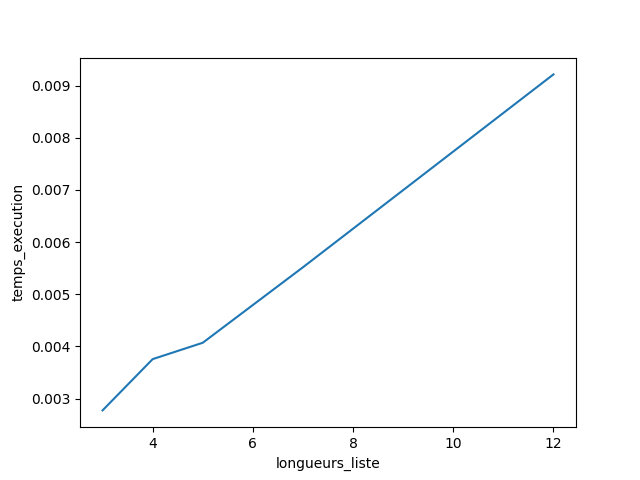
\includegraphics[scale=0.9]{figures/evaluation_test.png}
    \caption{Mesures du temps exécution en fonction de la longueur des mots}
    \label{fig:my_label}
\end{figure}
\newpage
\subsection{Fonction dicoload du solveur}
\subsubsection{Complexité théorique}
Soit p le nombre de mots du dictionnaire choisi, Cette fonction a une complexité temporelle en o($p$). La fonction dicoload du solveur a donc une complexité temporelle linéaire.

\subsection{Fonction evaluation du solveur}
\subsubsection{Complexité théorique}
Soit n la longueur des mots du dictionnaire choisi. Cette fonction a une complexité temporelle en o($n^2$). La fonction evaluation du solveur a donc une complexité temporelle quadratique.


\subsection{Fonction WordEntropy du solveur}
\subsubsection{Complexité théorique}
Soit p le nombre de mots du dictionnaire et n la longueur des mots; Cette fonction a une complexité temporelle en o(p * $n^2$).

\subsection{Fonction getbestword du solveur}
\subsubsection{Complexité théorique}
Soit p le nombre de mots du dictionnaire et n la longueur des mots; Cette fonction a une complexité temporelle en o($p^2$ * $n^2$).

\subsection{Fonction FindWordsGreen du solveur}
\subsubsection{Complexité théorique}
Soit p le nombre de mots du dictionnaire et n la longueur des mots; Cette fonction a une complexité temporelle en o($p$ * $n$).

\subsection{Fonction FindWordsYellow du solveur}
\subsubsection{Complexité théorique}
Soit p le nombre de mots du dictionnaire et n la longueur des mots; Cette fonction a une complexité temporelle en o($p$ * $n^2$).

\subsection{Fonction excludeWords du solveur}
\subsubsection{Complexité théorique}
Soit p le nombre de mots du dictionnaire et n la longueur des mots; Cette fonction a une complexité temporelle en o($p$ * $n^2$).

\subsection{Fonction MotsSuivantsPossibles du solveur}
\subsubsection{Complexité théorique}
Soit p le nombre de mots du dictionnaire et n la longueur des mots; Cette fonction a une complexité temporelle en o($p$ * $n^3$).

\newpage
\section{Gestion de projet}
\subsection{Membres de l'équipe}

\tabto{1cm}L'équipe projet est composée de 4 élèves : Armand LONDEIX, Lucas RIOUX, Patrick O'BRIEN et Serge TÉHÉ. Lucas est désigné chef de projet et aura la responsabilité de s'assurer de l'avancement global du projet.

\subsection{Organisation du projet}

\tabto{1cm}Le projet s'est déroulé du 23 mars 2022 au 8 juin 2022. L'équipe projet s'est réunie principalement sur Discord et à TELECOM Nancy pour les réunions, qui se tenaient généralement en début d'après-midi. Le projet a été scindé en deux sous-projets : d'une part, le \textbf{jeu WORDLE} (application Web, interface graphique, base de données) et d'autre part le \textbf{solveur}.

\subsection{Outils de travail}

\tabto{1cm}Pour réaliser notre projet, nous avons développé avec l'éditeur de code Visual Studio Code. Nous avons aussi utilisé GanttProject pour réaliser le diagramme de Gantt, Inkscape pour faire une maquette de l'interface graphique et des outils de bureautique tels qu'Excel pour la matrice RACI. Le rapport a été rédigé en \LaTeX{}. Le travail a été mis en commun sur le gitlab de l'école.

%\subsection{Partage du travail}

% Tout ce qui est dit ici est dit dans la RACI, je pense que ce paragraphe n'est pas utile -Lucas

%Pour le site web d'une part, Serge savait bien manipulé javascript contrairement aux autres membres du groupe il s'est donc chargé de la partie en javascript et de l'affichage en dynamique. Le reste des membres du groupes se sont occupé de la partie flask, des différentes fonction d'évaluation, des systèmes et comptes récompenses,... \\
%Pour la partie Solveur, Armand et Serge se sont occupés des fonctions qui permettent au solveur de fonctionner c'est à dire les fonction qui calculent l'entropie, qui testent les mots en fonction d'une combinaison,... Lucas et Patrick se sont occupés quant à eux de coder le solveur et de l'implémenter pour qu'il puisse fonctionner grâce aux fonctions d'Armand et Serge. \\

\subsection{Documents relatifs au projet}

\tabto{1cm}Différents documents de gestion de projet ont été réalisés, en plus des comptes-rendus, afin de retracer son déroulement : une matrice SWOT afin d'analyser les risques du projet, un WBS pour sééquencer les tâches, une matrice RACI attribuant les diffréntes tâches aux membres de l'équipe et un diagramme de Gantt rendant compte de l'avancement du projet. Tous ces documents sont en annexe.

\newpage
\subsection{Volume horaire}
\begin{figure}[h!]
    \centering
    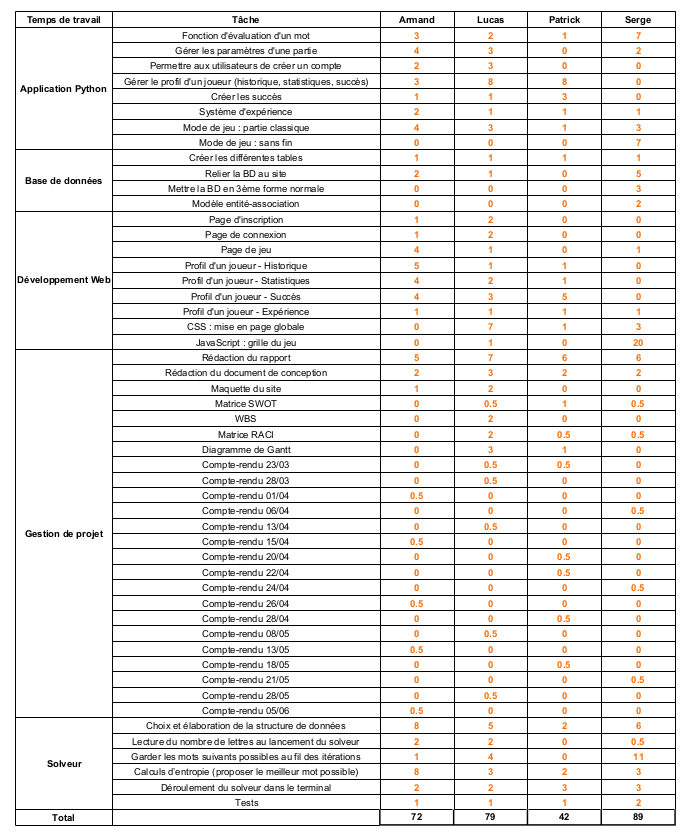
\includegraphics[width=16cm]{figures/Temps_travail.png}
    \caption{Volume horaire}
\end{figure}

\newpage

\section{Bilan du projet}
\subsection{Travail réalisé}

%Au cours de ce projet nous avons réalisé la conception et l'implémentation du jeu wordle en y intégrant  un système de compte utilisateur pour pouvoir enregistrer les parties, les scores,... Nous avons pu réaliser toutes les fonctions que nous avons imaginées au début du projet mais certaines idées qui nous venaient à la fin comme un mode de jeu contre la montre n'ont pu être implémenté faute de temps.\\
%Pour la partie solveur, nous avons créer un solveur en C qui permet effectivement lors de son utilisation de drastiquement réduire le nombre de coups utilisé. Le solveur est conforme à l'énoncé puisque qu'il trouve le mot optimal et qu'il renvoie la longueur du mot.

\tabto{1cm}Nous avons réussi à développer un jeu WORDLE paramétrable par le joueur (nombre d'essais, taille du mot, mode de jeu) avec un historique des parties et des fonctionnalités secondaires (succès, statistiques, expérience). Pour ce livrable, nous n'avons pas eu assez de temps pour créer un mode contre-la-montre, où le joueur aurait du deviner le maximum de mots en un temps donné.

\tabto{1cm}Le solveur est fonctionnel et réduit très vite l'ensemble des mots possibles pour converger vers la réponse : pour des mots comprenant de 4 à 8 lettres, la réponse est trouvée en 3 coups environ, et même en 2 coups pour des mots plus longs. Les livrables sont donc conformes aux attendus du projet.

\subsection{Bilan de l'équipe projet}

{\begin{center}
\begin{tabular}{|c|c|}
\hline Points positifs & - Implémentation des fonctions principales  \\
& - Renforcement des compétences de gestion de projet \\
\hline Points à améliorer & - Améliorer la communication au sein du groupe \\
& - Ne pas se concentrer sur les détails d'implémentation \\
& - Être plus efficace pendant les réunions \\
\hline Expérience collective & - Bonne impulsion de groupe \\
& - Utilisation de Gitlab \\
\hline
\end{tabular}
\end{center}}

\subsection{Bilan individuel}

\subsubsection{Armand Londeix} 
Dans la première partie du projet, je me suis impliqué dans l'interface Web, ainsi que dans la mise en place de certaines fonctions python, aussi cette partie m'a permis de consolider mes connaissances en HTML mais aussi de en m'impliquant dans la gestion du projet de m'améliorer en travail d'équipe, désormais je sais mieux comment renforcer l'organisation, la cohésion d'une équipe. \\
Dans la partie Solveur, le fait de coder en C m'a permis d'apprendre et de consolider mes connaissances dans un langage qui m'était nouveau, aussi je sais maintenant très bien utiliser les structures de données et coder en C n'est plus vraiment un problème. La collaboration avec mes camarades m'a permis de ne pas m'attarder sur certaines parties qui me posaient problèmes au début pour progresser dans mon travail. \\ 
Je garde un bon souvenir de ce projet tant sur le plan des connaissances que j'ai acquises que sur la gestion de projet et les relations avec mes camarades. \\ 
\subsubsection{Patrick O'Brien}
Ce projet m'a permis de développer ma programmation en algorithmes et en Web. J'ai appris à bien travailler en équipe. J'ai eu quelques problèmes dus à une mauvaise communication de ma part mais j'ai vu cela comme une opportunité de créer plus de cohésion dans le groupe. Il était très facile de travailler avec mes camarades et ils ont été très utiles pour résoudre les difficultés que j'ai rencontrées. En ce qui concerne le gestion de projet, je comprend bien l'importance d'une réunion efficace.
\\ 
 
\subsubsection{Lucas Rioux}

Ce projet m'a permis d'améliorer mes compétences en Python et en développement Web, notamment en CSS et en JavaScript ; et également de découvrir le langage C, qui m'a forcé à me montrer plus rigoureux. Certaines fonctions du projet m'ont mis à rude épreuve, comme la fonction éliminant les réponses impossibles dans le solveur.
J'ai également pu mettre en pratique mes connaissances en gestion de projet et je commence à comprendre comment travailler en équipe. Dans l'ensemble, je suis satisfait des autres membres de l'équipe ainsi que du travail effectué.

\subsubsection{Serge Téhé}
Ce projet m'a permi d'acquérir des connaissances plus poussées en algorithmique, en programmation Web et en langage C. J'ai pu développer tout au long du projet certaines aptitudes et réflexes en informatique et en gestion de projet qui me donnent ainsi une expérience de plus sur mon CV. Ce projet m'a aussi permis d'écouter les autres membres du groupe et de trouver un point commun de convergence des idées malgré nos divergences souvent très ostentatoires.



\newpage
\section{Annexe}

\subsection{Documents de gestion de projet}
\subsection*{Matrice SWOT}

\begin{figure}[h!]
    \centering
    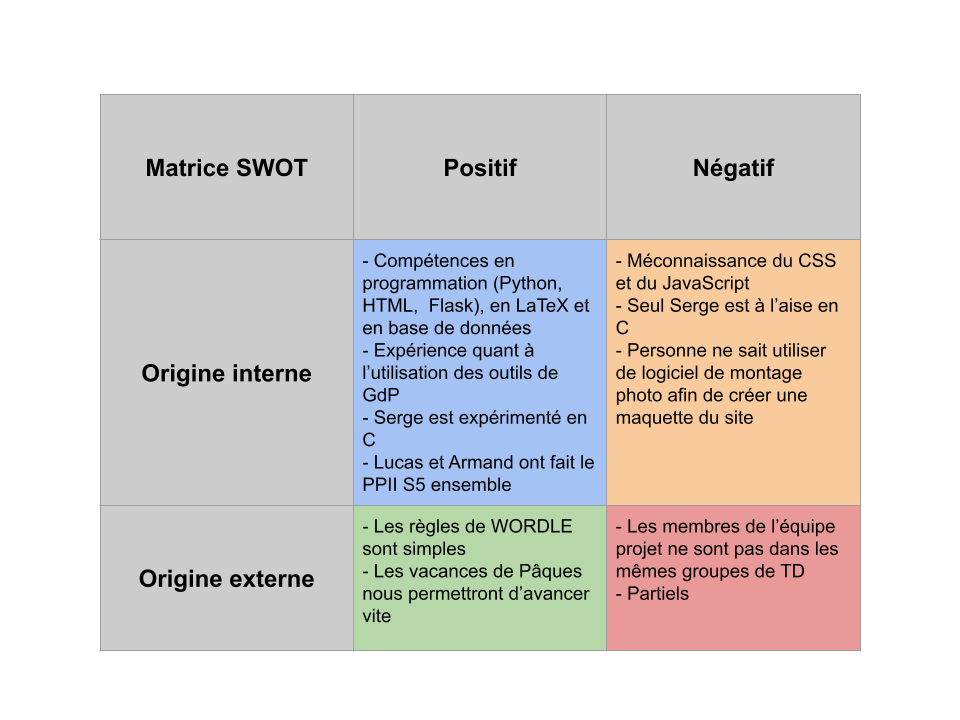
\includegraphics[width=16cm]{figures/SWOT.png}
    \caption{Matrice SWOT}
\end{figure}
\newpage
\subsection*{WBS}

\begin{figure}[h!]
    \centering
    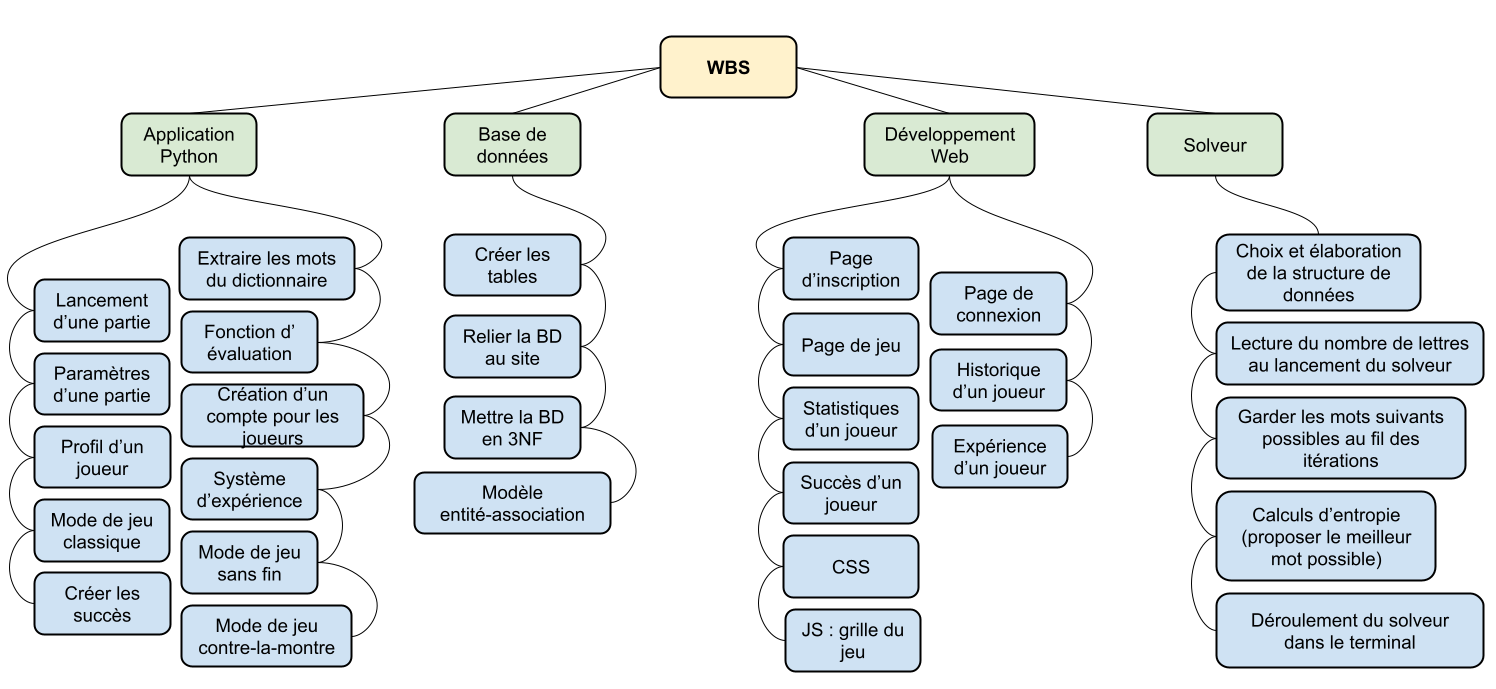
\includegraphics[width=16cm]{figures/WBS.png}
    \caption{WBS}
\end{figure}

\newpage
\subsection*{Matrice RACI}

\begin{figure}[h!]
    \centering
    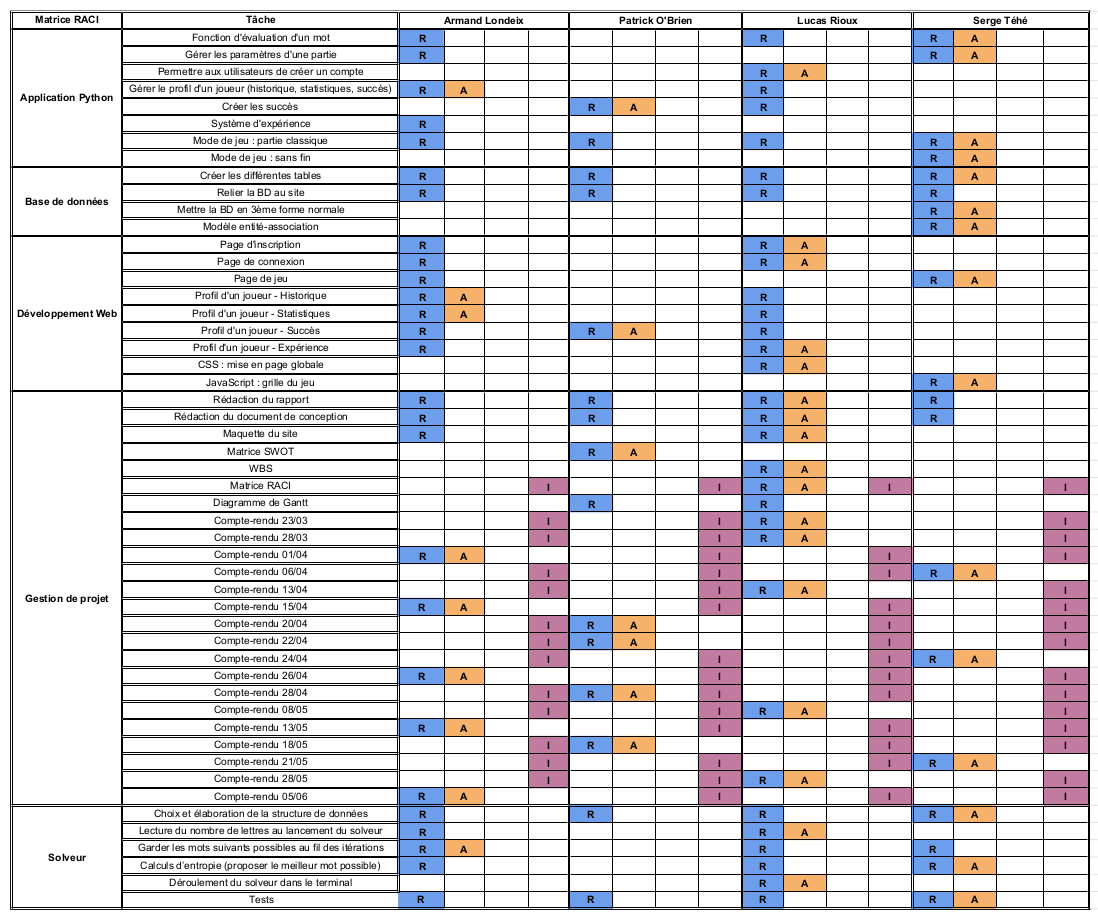
\includegraphics[width=16cm]{figures/RACI.png}
    \caption{Matrice RACI}
\end{figure}

\newpage

\subsection*{Diagramme de Gantt}

\begin{figure}[h!]
    \centering
    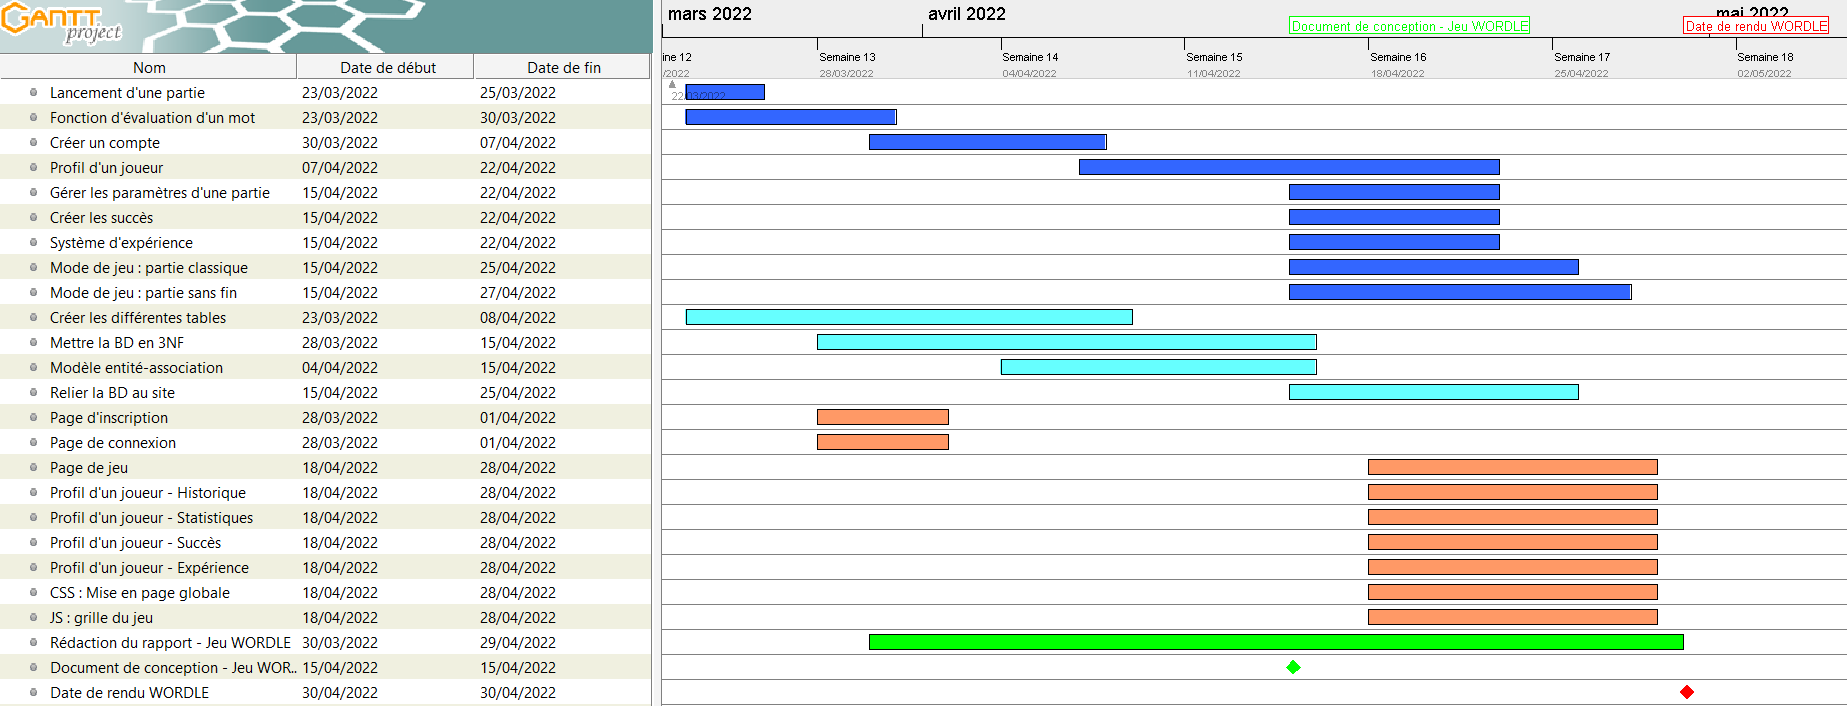
\includegraphics[width=18cm]{figures/gantt_jeu_wordle.PNG}
    \caption{Diagramme de Gantt - Jeu WORDLE}
\end{figure}

\begin{figure}[h!]
    \centering
    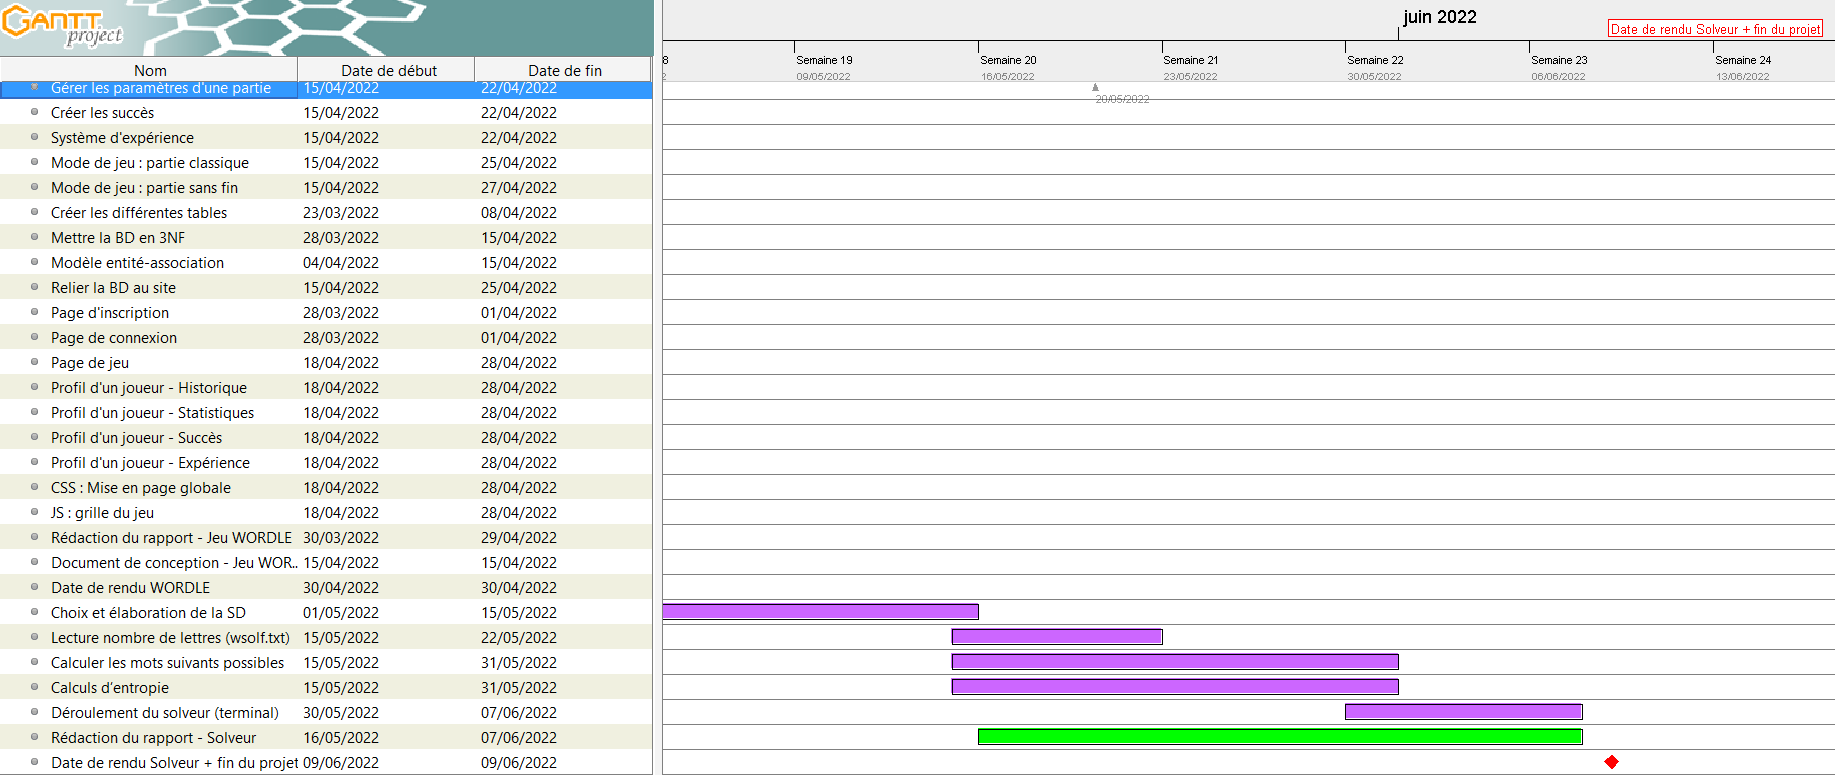
\includegraphics[width=18cm]{figures/gantt_solveur.PNG}
    \caption{Diagramme de Gantt - Solveur}
\end{figure}


\subsection{Comptes-rendus}

\subsubsection{Compte-rendu du 23 Mars 2022}
\begin{center}
\begin{tabular}[c]{|l|l|}
    \hline
    Type de réunion & Réunion d'avancement \\
    \hline
    Lieu & Telecom Nancy \\
    \hline
    Horaires & 16h00 - 17h30 \\
    \hline
    Maître de séance & Lucas Rioux\\
    \hline
    Secrétaires & Lucas Rioux, Patrick O'Brien \\
    \hline
    Membres présents & Armand Londeix \\ & Patrick O'Brien \\ & Lucas Rioux \\ & Serge Téhé\\
    \hline
    Membres absents & Aucun \\
    \hline
\end{tabular}
\end{center}

\section*{Ordre du jour}

\textbf{
\begin{enumerate}
    \item Atouts et faiblesses des membres du groupe
    \item Début du site : premières directives
    \item Éléments de gestion de projet
\end{enumerate}
}

\tabto{1cm}Avant le début de la réunion, le groupe a créé un groupe Messenger, un serveur Discord pour pouvoir communiquer, un Google Drive pour partager les documents relatifs au projet et un document Overleaf pour rédiger le rapport.

\section*{1. Atouts et faiblesses des membres du groupe}
\tabto{1cm}Lucas prend la parole et questionne les membres du groupe sur leurs compétences en matière de programmation (Python, SQL, HTML, CSS, Flask, C). Tous les membres du groupe affirment maîtriser Python, SQL, HTML et Flask mais moins le CSS. Concernant le C, seul Serge est expérimenté. Serge a d’ailleurs plus d’expérience avec l’utilisation de git car un module y était entièrement consacré l’année scolaire précédente.\\ \\
\tabto{1cm}Lucas propose d’utiliser les branches de git pour collaborer ensemble sans gêne et ne pas devoir prendre le risque de perdre du travail en commitant directement sur la branche master. Les autres membres du groupe sont d’accord avec cette idée, Lucas propose que tout le monde se renseigne sur ce point d’ici la prochaine réunion (cf. to-do list).
\\

\section*{2. Début du site : premières directives}
\tabto{1cm}Il est décidé que l’application sera implémentée grâce à la bibliothèque Flask de Python. À première vue, seulement deux pages HTML seront nécessaires : une page de connexion et une page avec le jeu. Patrick évoque la question de la gestion des caractères spéciaux, Lucas précise que ce problème est facilement gérable en Python.\\ \\
\tabto{1cm}Vient ensuite la question de la récupération des mots du dictionnaire français : ils ont été extraits de la base de données Lexique (version 3.83) (http://www.lexique.org/) par Lucas, répertoriant l’intégralité des mots français. L’ensemble des mots a été extrait vers un fichier texte, puis les doublons ont été supprimés. Armand a, quant à lui, récupéré des fichiers texte sur le github de ScienceEtonnante avec des mots déjà sélectionnés et séparés dans différents fichiers selon leur longueur. Il sera décidé plus tard de quel dictionnaire utiliser.

\section*{3. Éléments de gestion de projet}
\tabto{1cm}Les éléments de gestion de projet à rédiger dès maintenant sont la matrice SWOT et le diagramme de Gantt. Lucas propose aux membres du groupe de télécharger le logiciel gratuit Gantt Project permettant une création et mise à jour facile du diagramme de Gantt. Patrick se désigne pour réaliser la matrice SWOT et le début du diagramme de Gantt pour la prochaine réunion.

\section*{TO-DO LIST}

\begin{center}
\begin{tabular}{|c|l|}
    \hline
    Armand Londeix & - Se renseigner sur l’utilisation des branches de git \\
    & - Mettre en place l’environnement (Flask), \\
    & implémenter le début de l’application \\
    \hline
    Patrick O'Brien & - Se renseigner sur l’utilisation des branches de git \\ 
    & - Rédiger la matrice SWOT \\
    & - Commencer le diagramme de Gantt \\
   \hline
    Lucas Rioux & - Se renseigner sur l’utilisation des branches de git \\
    & - Extraire les mots de la base de données Lexique, \\
    & en supprimer les doublons \\
    \hline
    Serge Téhé & - Se renseigner sur l’utilisation des branches de git\\
    & - Extraire les mots de la base de données Lexique, \\
    & en supprimer les doublons \\
    \hline
\end{tabular}
\end{center}

\tabto{0cm}\textbf{Prochaine réunion : Lundi 28 Mars à 13h00.}

\subsubsection{Compte-rendu du 28 Mars 2022}
\begin{center}
\begin{tabular}[c]{|l|l|}
    \hline
    Type de réunion & Réunion d'avancement \\
    \hline
    Lieu & Telecom Nancy \\
    \hline
    Horaires & 13h00 - 14h00\\
    \hline
    Maître de séance & Lucas Rioux\\
    \hline
    Secrétaire & Lucas Rioux \\
    \hline
    Membres présents & Armand Londeix \\ & Patrick O'Brien \\ & Lucas Rioux \\ & Serge Téhé\\
    \hline
    Membres absents & Aucun \\
    \hline
\end{tabular}
\end{center}

\section*{Ordre du jour}

\textbf{
\begin{enumerate}
    \item Avancement depuis la dernière réunion
    \item Implémentation de l’application
\end{enumerate}
}

\tabto{1cm}Les membres du groupe ont tous téléchargé GanttProject en amont de la réunion. GanttProject est un logiciel gratuit permettant de créer un diagramme de Gantt.

\section*{1. Avancement depuis la dernière réunion}
\tabto{1cm}Depuis la précédente réunion, Lucas a obtenu des renseignements concernant d’autres bases de données contenant l’ensemble des mots du dictionnaire français, et notamment l’Officiel du Scrabble (ODS 6) avec presque 400 000 mots. L’équipe projet ne s’est pas encore prononcée sur la question du dictionnaire utilisé. Patrick a mis en place le début du diagramme de Gantt et les membres se sont renseignés sur l’utilisation des branches de git.\\

\section*{2. Implémentation de l’application}
\tabto{1cm}Il s'ensuit un débat pour savoir s’il faut ranger les mots dans un seul fichier texte, différents fichiers texte selon leur longueur ou bien dans une base de données (une table plus précisément). Serge et Armand sont partants pour préalablement trier les mots selon leur longueur dans un souci de gain de temps de calcul, ce sur quoi le groupe s’accorde.
En ce qui concerne la base de données, elle comporte pour l’instant deux tables :

\begin{center}
\begin{tabular}[c]{|l|l|}
    \hline
    \textbf{User} & \textbf{Historique} \\
    \hline
    \textbf{idUser} INTEGER, PRIMARY KEY & \textbf{idPartie} INTEGER, \\ & PRIMARY KEY \\
    \hline
    \textbf{pseudo} VARCHAR(20), UNIQUE & \textbf{idUser} INTEGER, \\ & FOREIGN KEY REFERENCES \\ & User(idUser) \\
    \hline
    \textbf{motDePasse} VARCHAR(20) & \textbf{motSecret} VARCHAR(15)\\
    \hline
    & \textbf{nbTentatives} INTEGER\\
    \hline
\end{tabular}
\end{center}

Lucas a rappelé que la base de données doit être en 3ème forme normale, et rappelle les règles (qui sont dans le cours). Pour l’instant, le groupe se demande s’il faut enregistrer uniquement la solution d’une partie et le nombre de coups joués pour gagner, ou bien s’il faut aussi sauvegarder l’ensemble des mots joués au cours d’une partie. Pour Armand, élaborer la base de données n’est pas une priorité : il faut se concentrer sur le développement Web. 
Plusieurs pages HTML sont envisagées :
\begin{itemize}
    \item index, la page d’accueil du site
    \item register et login, pour s’inscrire et se connecter,
    \item game, la page avec le jeu,
    \item history, pour voir l’historique de nos parties,
    \item success, pour voir nos succès dans le jeu.
\end{itemize}
Cette liste est évidemment non exhaustive. Aussi, un utilisateur devra impérativement être connecté pour jouer : cette fonctionnalité peut être implémentée avec les bibliothèques Flask-Session et Flask-Login.\\

\section*{TO-DO LIST}

\begin{center}
\begin{tabular}{|c|l|}
    \hline
    Armand Londeix & - Implémenter la page avec le jeu \\
    \hline
    Patrick O'Brien & - Réaliser une maquette du site sur Inkscape \\ 
    & - Commencer à rédiger le document de conception \\
   \hline
    Lucas Rioux & - Réaliser une maquette du site sur Inkscape \\
    \hline
    Serge Téhé & - Implémenter la page avec le jeu\\
    \hline
\end{tabular}
\end{center}

\tabto{0cm}\textbf{Prochaine réunion : Vendredi 1er Avril à 13h00.}

\subsubsection{Compte-rendu du 1er Avril 2022}
\begin{center}
\begin{tabular}[c]{|l|l|}
    \hline
    Type de réunion & Réunion d'avancement \\
    \hline
    Lieu & Telecom Nancy \\
    \hline
    Horaires & 13h00 - 14h00 \\
    \hline
    Maître de séance & Lucas Rioux\\
    \hline
    Secrétaire & Armand Londeix \\
    \hline
    Membres présents & Armand Londeix \\ & Patrick O'Brien \\ & Lucas Rioux \\ & Serge Téhé\\
    \hline
    Membres absents & Aucun \\
    \hline
\end{tabular}
\end{center}

\section*{Ordre du jour}

\textbf{
\begin{enumerate}
    \item Avancement depuis la dernière réunion et suppression de fichiers inutiles sur le git
    \item Élaboration de la base de données
\end{enumerate}
}


\section*{1. Avancement depuis la dernière réunion et suppression de fichiers inutiles sur le git}
\tabto{1cm}On compte prendre un nouveau dictionnaire, soit on garde celui d’Armand qui a l’avantage d’être trié par fréquence et constitue une grosse base de données, soit on prend celui de Lucas qui contient davantage de mots. De toute façon le changement du dictionnaire est relativement aisé et on pourra toujours revenir dessus. On décide donc de garder le dictionnaire d’Armand et de changer au cas où.

\section*{2. Élaboration de la base de données}
\tabto{1cm}On parle de la façon dont on organise le site, Lucas propose de créer un compte avant de pouvoir jouer, Armand pense qu’on peut jouer sans compte mais que dans ce cas là les achievements, les enregistrements de parties et autres fonctionnalités ne fonctionneraient pas, on va rester sur cette idée.

\tabto{1cm}Lucas pense qu’il faut supprimer la page succes qui ne sert pas à grand chose mais qui ne compromet pas le bon fonctionnement du site, il est décidé de revenir à ça plus tard.

\tabto{1cm}Pour tous se mettre d’accord, on fait sur un tableau le schéma du site ainsi que celui des bases de données.

\tabto{1cm}Pour la page de connexion Lucas propose de mettre juste un pseudo non pris, après réflexion on se demande s’il ne faut pas un mot de passe car certains joueurs pourraient jouer sur le compte d’autres.

\tabto{1cm}Pour la base de données, on créera 3 tables, une table utilisateur avec les noms d’utilisateur et les mots de passe et une table historique (utilisateur, nombre d'essai, mots utilisés,...), enfin une dernière table permettra de stocker les succès (victoires, victoires en moins de coups,...).

\section*{TO-DO LIST}

\begin{center}
\begin{tabular}{|c|l|}
    \hline
    Armand Londeix & - Continue la construction du site \\
    & - Page achievement, historique \\
    & - Base de données \\
    \hline
    Patrick O'Brien & - Document de conception \\ 
   \hline
    Lucas Rioux & - Mettre à jour la matrice RACI \\
    \hline
    Serge Téhé & - Gérer la fin du jeu \\
    & - evaluation de chaque lettre dans un mot \\
    & pour en associer des couleurs \\
    \hline
\end{tabular}
\end{center}

\tabto{0cm}\textbf{Prochaine réunion : Mercredi 6 Avril à 12h30.}

\subsubsection{Compte-rendu du 6 Avril 2022}
\begin{center}
\begin{tabular}[c]{|l|l|}
    \hline
    Type de réunion & Réunion d'avancement \\
    \hline
    Lieu & Telecom Nancy \\
    \hline
    Horaires & 12h30 - 13h20 \\
    \hline
    Maître de séance & Serge Téhé\\
    \hline
    Secrétaire & Serge Téhé \\
    \hline
    Membres présents & Armand Londeix \\ & Patrick O'Brien \\ & Lucas Rioux \\ & Serge Téhé\\
    \hline
    Membres absents & Aucun \\
    \hline
\end{tabular}
\end{center}

\section*{Ordre du jour}

\textbf{
\begin{enumerate}
    \item Architecture du site
    \item Élaboration de la base de données
    \item Présentation du jeu Wordle par Serge Téhé
\end{enumerate}
}


\section*{1. Architecture du site}
\tabto{1cm}Au début de la réunion, nous avons commencé par mettre en œuvre l’architecture de notre site Web.  Lucas s’est mis au tableau pour écrire toutes les propositions des membres du groupe et nous nous sommes mis d’accord sur plusieurs points.\\
\tabto{1cm}L’utilisateur non connecté arrivant sur la page d’accueil du site voit le jeu Wordle auquel il peut directement jouer sans être inscrit au préalable. Sur cette même page, cet utilisateur non connecté aperçoit au niveau de la barre de navigation principale un paramétrage pour paramétrer la longueur des mots et le nombre d’essais maximum puis 2 boutons d’inscription et de connexion. Ces boutons d’inscription et de connexion servent à enregistrer un joueur de sorte à ce qu’il puisse voir son historique de parties jouées et les niveaux qu’il a débloqués (hard,medium,easy).\\
\tabto{1cm}L’utilisateur connecté quant à lui peut voir son profil avec les niveaux débloqués ainsi que des boutons de déconnexion, de statistiques sur les anciennes parties jouées et aussi de paramétrage du jeu.\\
\tabto{1cm}Certains membres du groupe ont proposé d’autres fonctionnalités telles que le mot du jour, endless, contre-la -montre que nous implémenterons si nous avons le temps.


\section*{2. Élaboration de la base de données}
\tabto{1cm}La base de données permet d’enregistrer les données des utilisateurs connectés. Nous avons convenu la création de 3 tables :

\begin{center}
\begin{tabular}[c]{|l|l|l|}
    \hline
    \textbf{User} & \textbf{Historique} & \textbf{Succès} \\
    \hline
    idUser INTEGER PK & idPartie INTEGER PK & idSucces INTEGER PK \\
    pseudo STR & idUser INTEGER FK & idUser INTEGER FK \\
    motDePasse STR & nb\_essais STR & estObtenu BOOLEAN \\
    & longueurMot INTEGER & \\
    \hline
\end{tabular}
\end{center}

Cette base de données ressort de nos propositions, nous la normaliserons éventuellement en 3ème forme normale.


\section*{3. Présentation du jeu Wordle par Serge Téhé}
\tabto{1cm}Nous n’avons pas eu le temps pour cette partie, Serge devait présenter et expliquer son implémentation du jeu Wordle.

\section*{TO-DO LIST}

\begin{center}
\begin{tabular}{|c|l|}
    \hline
    Armand Londeix & - Rédaction du document de conception \\
    \hline
    Patrick O'Brien & - Rédaction du document de conception \\
    & - Présentation textuelle du jeu Wordle \\
    \hline
    Lucas Rioux & - Maquette du site \\
    & - WBS \\
    & - Rédaction du document de conception \\
    \hline
    Serge Téhé & - Normalisation de la base de données \\
    & - Rédaction du document de conception \\
    \hline
\end{tabular}
\end{center}

\tabto{0cm}\textbf{Prochaine réunion : Mercredi 13 Avril à 14h00.}

\subsubsection{Compte-rendu du 13 Avril 2022}
\begin{center}
\begin{tabular}[c]{|l|l|}
    \hline
    Type de réunion & Réunion d'avancement \\
    \hline
    Lieu & Discord \\
    \hline
    Horaires & 14h00 - 15h00 \\
    \hline
    Maître de séance & Lucas Rioux\\
    \hline
    Secrétaire & Lucas Rioux \\
    \hline
    Membres présents & Armand Londeix \\ & Patrick O'Brien \\ & Lucas Rioux \\ & Serge Téhé\\
    \hline
    Membres absents & Aucun \\
    \hline
\end{tabular}
\end{center}

\section*{Ordre du jour}

\textbf{
\begin{enumerate}
    \item Avancement depuis la dernière réunion
    \item Fonction evaluation(), jeu WORDLE : clarification
    \item Base de données de l’application
    \item Mise en place du CSS
\end{enumerate}
}


\section*{1. Avancement depuis la dernière réunion}
\tabto{1cm}Au début de la réunion, il a été décidé à 3 votes contre un de supprimer la route /dico ainsi que la page dico.html, jugés inutiles à l’application. Ensuite, chacun des membres de l’équipe projet fait un bilan sur ce qui a été réalisé depuis la dernière réunion :

\begin{itemize}
\item Armand a commencé à développer la page achievements.html renommée ensuite en profile.html. Il a rencontré certains problèmes avec notamment un module non installé (pytest) qui ne lui permettait pas de lancer l’application via flask run, et aussi avec le dictionnaire session. Ces problèmes ont été résolus.
\item Patrick a rédigé une partie du document de conception concernant la base de données et le site HTML : Lucas lui fait remarquer qu’il devait s’occuper de la présentation textuelle du jeu, ce que Patrick note et fera pour la prochaine réunion. Il rencontre des soucis avec la commande git pull, a priori résolus.
\item Serge s’est chargé de concevoir et de normaliser en 3ème forme normale la base de données. Il s’occupera ensuite du modèle entité-association.
\item Lucas a réalisé une première maquette du site Web, un schéma de ses routes ainsi qu’un schéma de son architecture. Il a aussi fait le WBS et ajouté le README sur le git.
\end{itemize}

\section*{2. Fonction evaluation(), jeu WORDLE : clarification}
\tabto{1cm}Lucas a retiré sa fonction evaluation() pour laisser celle d’Armand, qui avait implémenté cette fonctionnalité le premier.\\
Vient ensuite une question cruciale : quelle application utiliser ? Armand, \tabto{1cm}Patrick et Lucas ont, pour le début du développement, mis en place un formulaire tandis que Serge a développé l’entièreté du jeu de son côté (fonction d’évaluation, mise en forme) en JavaScript, langage que seul lui maîtrise. Armand propose à Serge d’essayer de “remplacer” le code Python sur la route “/” en JavaScript, ou d’essayer d’établir une connexion entre les deux fichiers afin de conserver les fonctions déjà développées. Serge lui répond que c’est impossible.\\ 
\tabto{1cm}Concernant le mot secret, le problème ne se pose pas puisqu’il est déclaré dans app.py. Afin de relier le fichier JavaScript et la base de données, Serge propose de faire du web scraping. Serge accepte de se charger de la connexion entre le fichier JavaScript et la base de données.\\

\section*{3. Base de données de l’application}
\tabto{1cm}Serge nous présente son travail sur la base de données du site. Suite à des discussions ayant eu lieu après la réunion, la base de données retenue est la suivante :\\ \\ \\ \\ \\ \\ \\

\begin{figure}[h!]
\centering
\includegraphics[width=12cm]{figures/bddfinalnormalisé.png}
\caption{Schéma de la base de données de WORDLE}
\end{figure}

\section*{4. Mise en place du CSS}
\tabto{1cm}Enfin, Lucas rappelle au groupe qu’il faudrait commencer à mettre en forme le site. Armand veut bien commencer à s’en charger.

\section*{TO-DO LIST}

\begin{center}
\begin{tabular}{|c|l|}
    \hline
    Armand Londeix & - Rédaction du document de conception \\
    \hline
    Patrick O'Brien & - Rédaction du document de conception \\
    & - Présentation textuelle du jeu Wordle \\
    \hline
    Lucas Rioux & - Maquette du site \\
    & - WBS \\
    & - Rédaction du document de conception \\
    \hline
    Serge Téhé & - Normalisation de la base de données \\
    & - Rédaction du document de conception \\
    \hline
\end{tabular}
\end{center}

\tabto{0cm}\textbf{Prochaine réunion : Vendredi 15 Avril à 10h00.}

\subsubsection{Compte-rendu du 15 Avril 2022}
\begin{center}
\begin{tabular}[c]{|l|l|}
    \hline
    Type de réunion & Stand-up meeting \\
    \hline
    Lieu & Discord \\
    \hline
    Horaires & 14h00 - 14h30 \\
    \hline
    Maître de séance & Lucas Rioux\\
    \hline
    Secrétaire & Armand Londeix \\
    \hline
    Membres présents & Armand Londeix \\ & Lucas Rioux \\ & Serge Téhé\\
    \hline
    Membres absents & Patrick O'Brien \\
    \hline
\end{tabular}
\end{center}

\section*{Ordre du jour}

\textbf{
\begin{enumerate}
    \item Ce qui a été fait
    \item Validation du document de conception
\end{enumerate}
}

\section*{1. Ce qui a été fait}
\tabto{1cm}Armand nous explique que le site a été mis à jour, désormais il est possible de modifier les paramètres de jeu, aussi un clic sur le bouton home permet de remettre à zéro la partie, enfin la page statistique est au point. \\

\tabto{1cm}Serge et Lucas se sont concentrés sur la base de données et le document de conception, ils conseillent à Armand d’utiliser la propriété "AUTOINCREMENT" dans la base de données pour faciliter le remplissage des clés primaires des différentes tables. Serge a notamment normalisé la base de données. \\ 
\tabto{1cm}Lucas s’est concentré sur la base de données ainsi que le Wbs et la conception de la maquette. \\ \\

\section*{2. Validation du document de conception}
\tabto{1cm}Le document de conception est au point, Serge remarque qu’on aurait dû le faire plus tôt ceci dit ce n’est pas trop grave : ça nous aurait juste fait perdre du temps.
Nous vérifions surtout que tout le monde est d’accord avec la conception du site et la partie CSS avant de pouvoir l’envoyer à M.Festor pour la faire valider, Patrick nous a d’ores et déjà donné son approbation. \textbf{On attend la validation du document de conception pour donner quelque chose à faire à Patrick.}

\section*{TO-DO LIST}

\begin{center}
\begin{tabular}{|c|l|}
    \hline
    Armand Londeix & - Rédiger le compte rendu \\
    \hline
    Patrick O'Brien & - Aucune tâche \\
    \hline
    Lucas Rioux & - Mettre à jour le Gantt \\
    \hline
    Serge Téhé & - Expliquer comment implémenter le jeu \\
    & sur le site sur le document de conception \\
    \hline
\end{tabular}
\end{center}

\tabto{0cm}\textbf{Prochaine réunion : Mercredi 20 Avril à 14h00.}

\subsubsection{Compte-rendu du 20 Avril 2022}
\begin{center}
\begin{tabular}[c]{|l|l|}
    \hline
    Type de réunion & Stand-up meeting \\
    \hline
    Lieu & Discord \\
    \hline
    Horaires & 14h30 - 14h50 \\
    \hline
    Maître de séance & Lucas Rioux\\
    \hline
    Secrétaire & Armand Londeix \\
    \hline
    Membres présents & Armand Londeix \\ & Patrick O'Brien \\ & Lucas Rioux \\ & Serge Téhé\\
    \hline
    Membres absents & Aucun \\
    \hline
\end{tabular}
\end{center}

\section*{Ordre du jour}

\textbf{
\begin{enumerate}
    \item Parler du document de conception et de ce qui a été fait
\end{enumerate}
}

\section*{1. Parler du document de conception et de ce qui a été fait}

\begin{itemize}
    \item Tout le monde est d’accord avec ce qu’on a mis dans le document de conception et maintenant on attend la réponse de M. Festor ;
    \item Lucas a réalisé le Gantt ;
    \item Lucas pense qu’il faut faire une réunion tous les deux jours. Armand est d’accord mais préférerait des réunions assez courtes avec une réunion d’avancement longue moins fréquente. Tout le monde décide finalement de faire des réunions courtes (stand-up meetings) tous les deux jours de 10-15 minutes ;
    \item Tout le monde est d’accord que c’est trop tard d’ajouter des nouvelles fonctionnalités ;
    \item Lucas a commencé à apprendre le JavaScript. Armand pense que JavaScript est moins documenté en ligne du coup il faut minimiser le nombre de fichiers JavaScript. Il demande à Serge, qui a le plus d’expérience en JavaScript, s’il sait faire certains trucs en JavaScript ;
    \item Lucas demande comment récupérer le nombre de tentatives, Serge dit qu’il a une idée qu’il peut essayer.

\end{itemize}

\section*{TO-DO LIST}

\begin{center}
\begin{tabular}{|c|l|}
    \hline
    Armand Londeix & - Implémenter l'historique des parties \\
    & et des statistiques \\
    \hline
    Patrick O'Brien & - Créer les achievements \\
    & Rédiger les CRs en \LaTeX{} \\
    \hline
    Lucas Rioux & - Commencer le CSS \\
    \hline
    Serge Téhé & - Remplir le fichier .sql (pour créer la BD) \\
    & Modèle entité-association \\
    \hline
\end{tabular}
\end{center}

\tabto{0cm}\textbf{Prochaine réunion : Vendredi 22 Avril à 11h00.}

\subsubsection{Compte-rendu du 22 Avril 2022}
\begin{center}
\begin{tabular}[c]{|l|l|}
    \hline
    Type de réunion & Stand-up meeting \\
    \hline
    Lieu & Discord \\
    \hline
    Horaires & 11h00 - 11h30 \\
    \hline
    Maître de séance & Lucas Rioux\\
    \hline
    Secrétaire & Patrick O'Brien \\
    \hline
    Membres présents & Armand Londeix \\ & Patrick O'Brien \\ & Lucas Rioux \\ & Serge Téhé\\
    \hline
    Membres absents & Aucun \\
    \hline
\end{tabular}
\end{center}

\section*{Ordre du jour}

\textbf{
\begin{enumerate}
    \item Parler de ce qui a été fait
\end{enumerate}
}

\section*{1. Parler de ce qui a été fait}

\begin{itemize}
    \item Lucas a bien développé le CSS du site ;
    \item Armand a travaillé sur l’historique et les statistiques. Il avait toujours une petite erreur avec la fonction ‘fetchone()’ mais on pense qu’il va la résoudre bientôt ;
    \item Patrick a fait une liste des achievements possibles et il a rédigé le premier compte-rendu en \LaTeX{}. Il a fait aussi une fonction démo pour calculer les achievements en utilisant les données dans la table ‘Partie’ mais on a décidé de mettre les achievements dans un autre table 'AchievementDesc' ;
    \item Serge a mis à jour le fichier databse.sql et a réalisé le modèle entité-association.
\end{itemize}

\section*{TO-DO LIST}

\begin{center}
\begin{tabular}{|c|l|}
    \hline
    Armand Londeix & - Implémenter l'historique des parties \\
    & et des statistiques \\
    \hline
    Patrick O'Brien & - Implémenter les succès \\
    & - Mettre leur description dans la BD \\

    \hline
    Lucas Rioux & - Rédiger les CRs en \LaTeX{} \\
    & - Finir le système d'inscription / de connexion \\
    \hline
    Serge Téhé & - Paramétrage de la grille selon \\
    & la longueur du mot et le nombre d'essais maximum \\
    \hline
\end{tabular}
\end{center}

\tabto{0cm}\textbf{Prochaine réunion : Dimanche 24 Avril à 14h00.}

\subsubsection{Compte-rendu du 24 Avril 2022}
\begin{center}
\begin{tabular}[c]{|l|l|}
    \hline
    Type de réunion & Réunion d'avancement \\
    \hline
    Lieu & Telecom Nancy \\
    \hline
    Horaires & 12h30 - 13h20 \\
    \hline
    Maître de séance & Serge Téhé\\
    \hline
    Secrétaire & Serge Téhé \\
    \hline
    Membres présents & Patrick O'Brien \\ & Lucas Rioux \\ & Serge Téhé\\
    \hline
    Membres absents & Armand Londeix  \\
    \hline
\end{tabular}
\end{center}

\section*{Ordre du jour}

\textbf{
\begin{enumerate}
    \item Présentation des tâches accomplies
    \item Discussion à propos de la page "index.html"
\end{enumerate}
}

\section*{1. Présentation des tâches accomplies}
Au début de la réunion, Patrick pose des questions d'éclaircissement sur les tâches qu'il devrait accomplir qui concernent la fonction Achievement et l'insertion des descriptions dans la table.Lucas prend la parole et lui répond en lui faisant la remarque que l'idsucces en particulier et tous les identifiants devraient être supérieurs à 1. 
Patrick n'a donc pas terminé ses tâches, il devrait les finir pour la prochaine réunion.

Ensuite Serge prend la parole et présente la tâche qu'il devrait effectuer : le paramétrage de la grille Wordle; Il explique qu'il a réussit sa tâche et a aussi reglé les bugs au niveau du jeu car Lucas après avoir revérifié le jeu, s'est aperçu d'un bug. En outre, il affirme avoir entammé une autre tâche qui est la liaison des informations des joueurs et la base de donnée qu'il a aussi réussit et qu'il mettra sur le dépôt git après la réunion.

Enfin Lucas explique qu'il a aussi accompli toutes ses tâches à savoir la rédaction de certains comptes rendus en latex, le règlement des bugs au niveau de la page d'inscription.


\section*{2. Discussion à propos de la page "index.html"}

Serge affirme que le jeu ne fonctionne pas sur la route générant le fichier "index.html" à cause des formulaires qui ont été faits par Armand.

Lucas répond qu'il s'en occupera et va réamenager cette route de sorte à ce que le jeu fonctionne. 

Serge propose aussi de permettre qu'un utilisateur non connecté puisse pouvoir paramétrer la grille; Lucas répond: oui pourquoi pas? Serge réaffirme: oui ou non? Lucas se décide finalement et aquiesce cette idée.




\section*{TO-DO LIST}

\begin{center}
\begin{tabular}{|c|l|}
    \hline
    Armand Londeix & - Continuer la page Profile \\
    \hline
    Patrick O'Brien 
    & - Continuer les succès et la fonction Achievement \\
    \hline
    Lucas Rioux & - permmettre à l'utilisateur non connecté de paramétrer la grille \\
    & - Intégrer le jeu sur la page "index.html" \\
    \hline
    Serge Téhé & - Prendre en compte les points d'expérience dans la base de donnée \\
    & - Liaison de la base de donnée avec 
    les informations des joueurs  \\
    \hline
\end{tabular}
\end{center}

\tabto{0cm}\textbf{Prochaine réunion : Mardi 26 Avril à 19h00.}

\subsubsection{Compte-rendu du 26 Avril 2022}
\begin{center}
\begin{tabular}[c]{|l|l|}
    \hline
    Type de réunion & Stand-up meeting \\
    \hline
    Lieu & Discord \\
    \hline
    Horaires & 19h00 - 19h30 \\
    \hline
    Maître de séance & Lucas Rioux\\
    \hline
    Secrétaire & Armand Londeix \\
    \hline
    Membres présents & Armand Londeix \\ & Lucas Rioux \\ & Serge Téhé\\ & Patrick O'Brien \\
    \hline
    Membres absents & Aucun \\
    \hline
\end{tabular}
\end{center}

\section*{Ordre du jour}

\textbf{
\begin{enumerate}
    \item Ce qui a été fait
    \item Validation du document de conception
\end{enumerate}
}

\section*{1. Ce qui a été fait}

\tabto{1cm}Armand a du mal en JavaScript et n’a pas réussi à implémenter les modes de jeu, cependant il a fait des grades ainsi qu’une barre de progression sur la page profile.html, après discussion on va les remplacer par des niveaux. Enfin l'historique est implémenté mais il reste du travail à faire, ce sera fini dans la soirée. \\

Patrick a fait la fonction achievements qui est bientôt finie. \\

Lucas a fait le CSS et a mis en \LaTeX{} les comptes-rendus. \\ \\
Serge a travaillé sur la base de données et leurs liens avec le site sur JavaScript.
 \\ \\

\section*{TO-DO LIST}

\begin{center}
\begin{tabular}{|c|l|}
    \hline
    Armand Londeix & - Faire les succès et éventuellement trouver des images \\ 
    \hline
    Patrick O'Brien & - Finir la fonction achievements \\
    \hline
    Lucas Rioux & - Continuer le CSS \\
    & - Finir l'historique \\
    \hline
    Serge Téhé & - Faire les modes de jeu \\
    \hline
\end{tabular}
\end{center}

\tabto{0cm}\textbf{Prochaine réunion : Jeudi 28 Avril à 12h00.}


\subsubsection{Compte-rendu du 28 Avril 2022}
\begin{center}
\begin{tabular}[c]{|l|l|}
    \hline
    Type de réunion & Stand-up meeting \\
    \hline
    Lieu & Discord \\
    \hline
    Horaires & 14h10 - 14h30 \\
    \hline
    Maître de séance & Lucas Rioux\\
    \hline
    Secrétaire & Patrick O'Brien \\
    \hline
    Membres présents & Armand Londeix \\ & Lucas Rioux \\ & Serge Téhé\\ & Patrick O'Brien \\
    \hline
    Membres absents & Aucun \\
    \hline
\end{tabular}
\end{center}

\section*{Ordre du jour}

\textbf{
\begin{enumerate}
    \item Avancement depuis la dernière réunion
    \item Ce qu'il reste à faire
\end{enumerate}
}

\section*{1. Avancement depuis la dernière réunion}

\begin{itemize}
    \item Serge a fait un mode de jeu "Sans fin" où un nouveau mot est proposé au joueur tant qu'il gagne : la partie s'arrête au premier mot non trouvé ;
    \item Armand a résolu quelques bugs et a trouvé quelques images pour les achievements ;
    \item Patrick a complété une fonction qui met à jour les achievements mais il y avait quelques bugs, Lucas a créé une autre fonction qui marche beaucoup plus mieux ;
    \item Lucas a aussi mis les CR en \LaTeX{} et fait un peu de CSS pour la page de profil.
\end{itemize}

\section*{2. Ce qu'il reste à faire}

\tabto{1cm}Tout le monde est d’accord qu'il ne nous reste pas beaucoup de tâches.
Serge pense que c’est important de jouer le jeu plusieurs fois afin de trouver des bugs.
Il faut choisir un logo, établir les niveaux d’expérience, tirer les mots les plus fréquents, tester la fonction d’évaluation et rendre le code plus propre.

\section*{TO-DO LIST}

\begin{center}
\begin{tabular}{|c|l|}
    \hline
    Armand Londeix & - Compléter la matrice RACI \\ 
    & - Tirer le mot à deviner parmi les mots les plus \\
    & - fréquents du dictionnaire (cf. dico science\_etonnante) \\
    \hline
    Patrick O'Brien & - Compléter la matrice RACI \\
    & - Implémenter le système d'expxérience \\
    \hline
    Lucas Rioux & - Compléter la matrice RACI \\
    & - Trouver un logo et une icône \\
    \hline
    Serge Téhé & - Compléter la matrice RACI \\
    & - Tests en JavaScript de la fonction d'évaluation de \emph{dash.js} \\
    \hline
\end{tabular}
\end{center}

\tabto{0cm}\textbf{Oral le Samedi 30 Avril à 10h00.}


\subsubsection{Compte-rendu du 8 mai 2022}
\begin{center}
\begin{tabular}[c]{|l|l|}
    \hline
    Type de réunion & Réunion d'avancement \\
    \hline
    Lieu & Telecom Nancy \\
    \hline
    Horaires & 14h00 - 15h00 \\
    \hline
    Maître de séance & Lucas Rioux\\
    \hline
    Secrétaire & Lucas Rioux \\
    \hline
    Membres présents & Armand Londeix \\ & Patrick O'Brien \\ & Lucas Rioux \\ & Serge Téhé\\
    \hline
    Membres absents & Aucun \\
    \hline
\end{tabular}
\end{center}

\section*{Ordre du jour}

\textbf{
\begin{enumerate}
    \item Mise au point : comment fonctionne le solveur en théorie
\end{enumerate}
}


\section*{1. Mise au point : comment fonctionne le solveur en théorie}

\tabto{1cm}Le groupe se met d’accord sur comment fonctionne le solveur en théorie et règle les soucis de compréhension après avoir visionné la vidéo de 3Blue1Brown https://www.youtube.com/watch?v=v68zYyaEmEA. 

\tabto{1cm}Le joueur devra obligatoirement jouer le mot proposé par le solveur sans quoi il risque d’échouer (conformément au sujet), ce que Armand confirme.

\tabto{1cm}La question de la structure de données utilisée pour stocker le dictionnaire se pose : pour l’instant, seule une liste (chaînée ou contiguë) est envisagée, étant donnée que le groupe n’arrive pas à comprendre comment utiliser un arbre pour résoudre ce problème bien que cette option semble efficace du point de vue de la complexité.

\tabto{1cm}Patrick demande ce qui se passe si l’utilisateur rentre une mauvaise combinaison de couleurs : dans ce cas, le solveur échouera. De toute manière, le solveur ne connaissant pas le mot à trouver, il suffira simplement de le relancer.

\tabto{1cm}Patrick demande aussi s’il sera possible de jouer (sur l’interface Web donc) un autre mot que celui proposé par le solveur : pour l’instant, cette option n’est pas envisagée.


\section*{TO-DO LIST}

\begin{center}
\begin{tabular}{|c|l|}
    \hline
    Armand Londeix & - Coder en C pour le solveur \\
    & - Rapport : rédiger l’historique et les statistiques \\
    \hline
    Patrick O'Brien & - Rapport : rédiger l’introduction, l’expérience et les achievements \\ 
    \hline
    Lucas Rioux & - Mettre les CR dans le rapport \\
    & - Rapport : agencement du site \\
    \hline
    Serge Téhé & - Complexité : fonction d’évaluation de index.js \\
    & - Rapport : rédiger la partie sur la base de données \\

    \hline
\end{tabular}
\end{center}

\tabto{0cm}\textbf{Prochaine réunion : Vendredi 13 mai à 13h00.}

\subsubsection{Compte-rendu du 13 mai 2022}
\begin{center}
\begin{tabular}[c]{|l|l|}
    \hline
    Type de réunion & Réunion d'avancement \\
    \hline
    Lieu & Discord \\
    \hline
    Horaires & 13h-13h30 \\
    \hline
    Maître de séance & Lucas Rioux\\
    \hline
    Secrétaire & Armand Londeix \\
    \hline
    Membres présents & Armand Londeix \\ & Lucas Rioux \\ & Serge Téhé\\ & Patrick O'Brien \\
    \hline
    Membres absents & Aucun \\
    \hline
\end{tabular}
\end{center}

\section*{Ordre du jour}

\textbf{
\begin{enumerate}
    \item Ce qui a été fait
    \item Todo list
\end{enumerate}
}

\section*{1. Ce qui a été fait}

\tabto{1cm}Armand a du mal en c à cause des listes et des structures pour stocker du texte mais est à l'aise avec l'idée du solveur, le rapport n'est pas encore fini. Quelques fonctions ont été crées et sont sur Gitlab cependant certaines sont inachevées. \\

Patrick a fait une partie du rapport mais avait des doutes sur le solveur, il a profité de la réunion pour poser des questions. \\

Lucas a avancé sur le solveur en python pour comprendre le principe du solveur en général. \\ \\
Serge a travaillé sur les structures pour stocker les mots.
 \\ \\

\section*{TO-DO LIST}
\tabto{1cm}Pour la prochaine fois nous allons faire ce qui n'a pas été fait pour la réunion et tous ensemble réfléchir sur le type de structure à implémenter pour les données avant de s'attaquer au solveur en tant que tel.
 \\ 
 Aussi nous allons par message nous tenir informé et essayer de déterminer avant ce week end la structure des données afin de commencer le solveur avant la prochaine réunion.
  \\ \\


\tabto{0cm}\textbf{Prochaine réunion : Mercredi 18 mai à 13h.}


\subsubsection{Compte-rendu du 18 mai 2022}
\begin{center}
\begin{tabular}[c]{|l|l|}
    \hline
    Type de réunion & Réunion d'avancement \\
    \hline
    Lieu & Discord \\
    \hline
    Horaires & 13h00 - 13h40 \\
    \hline
    Maître de séance & Lucas Rioux\\
    \hline
    Secrétaire & Patrick O'Brien \\
    \hline
    Membres présents & Armand Londeix \\ & Lucas Rioux \\ & Serge Téhé\\ & Patrick O'Brien \\
    \hline
    Membres absents & Aucun \\
    \hline
\end{tabular}
\end{center}

\section*{Ordre du jour}

\textbf{
\begin{enumerate}
    \item Ce qui a été fait
\end{enumerate}
}

\section*{1. Ce qui a été fait}

\begin{itemize}
    \item Lucas et Patrick ont bossé sur la rapport;
    \item Armand a bossé sur des listes chaînées, il pensait que des listes chaînées ne peuvent pas avoir des mots, Serge n’est pas d’accord, il sait le faire. Lucas dit que on peut stocker les mots dans un arbre binaire mais c’est compliqué;
    \item Serge pensait qu’une table des hash codes des mots peut être utile. On met les mots avec le même hashcode dans la même liste. Les autres du groupe avaient un peu du mal à comprendre exactement ce qu’il voulait faire avec cette table mais on est d’accord que c’est la meilleure façon de stocker les mots. ;
    \item Serge a réussi à récupérer le dictionnaire en faisant ça. Il a fait aussi une fonction (en python) pour calculer l’entropie de chaque mot;
    \item Tout le monde a décidé de se renseigner sur le TP de hachage. 
\end{itemize}

\section*{TO-DO LIST}

\begin{center}
\begin{tabular}{|c|l|}
    \hline
    Armand Londeix & - Se renseigner sur les tables de hachage, rapport, fichier wsolf.txt (lire longueur des mots) \\
    \hline
    Patrick O'Brien & - Se renseigner sur les tables de hachage, rapport \\ 
   \hline
    Lucas Rioux & - Se renseigner sur les tables de hachage, rapport \\
    \hline
    Serge Téhé & - Se renseigner sur les tables de hachage \\
    \hline
\end{tabular}
\end{center}

\tabto{0cm}\textbf{Prochaine réunion : Samedi 21 Mai à 17h00.}

\subsubsection{Compte-rendu du 21 mai 2022}
\begin{center}
\begin{tabular}[c]{|l|l|}
    \hline
    Type de réunion & Réunion d'avancement \\
    \hline
    Lieu & Discord \\
    \hline
    Horaires & 17h00 - 18h00 \\
    \hline
    Maître de séance & Serge Téhé \\
    \hline
    Secrétaire & Serge Téhé \\
    \hline
    Membres présents & Patrick O'Brien \\ & Lucas Rioux \\ & Serge Téhé\\ & Armand Londeix\\
    \hline
\end{tabular}
\end{center}

\section*{Ordre du jour}

\textbf{
\begin{enumerate}
    \item Présentation des tâches accomplies et Discussion à propos du dictionnaire à choisir
    \item  Réglages bugs Armand
\end{enumerate}
}

\section*{1. Présentation des tâches accomplies}

Au début de la réunion, chaque membre a presenté les tâches qu'il a accomplit.

Lucas a avancé sur le rapport,  en particulier sur la partie préentation de l'interface web qu'il devrait finaliser. 

Ensuite Patrick prend la parole pour poser une question relative au fonctionnement du solveur, il demande si on utilise le dictionnaire des mots les plus fréquents ou le dictionnaire des mots autorisés. Tous les membres répondent qu'on travaille sur le dictionnaire des mots fréquents. En outre, Patrick propose une stratégie de jeu qui consiste à choisir le mot le plus fréquent parmi les possibilités lorsque le solveur ne trouve pas le mot au bout d'un grand nombre d'essais.

Finalement Serge prend la parole et présente l'implémentation de la structure de données qu'on utilisera dans notre solveur.

\section*{2. Réglages bugs Armand}
Pendant la réunion, Armand a présenté un bug qu'il rencontrait au niveau de la table de hachage et Serge l'a aidé à trouvé le bug.

\section*{TO-DO LIST}

\begin{center}
\begin{tabular}{|c|l|}
    \hline
    Armand Londeix & - Calcul de probabilités \\
    \hline
    Patrick O'Brien 
    & - Expliquer les règles du jeu dans le rapport \\
    \hline
    Lucas Rioux & - Fonction d'écriture et de lecture fichier wsolf.txt  \\
    \hline
    Serge Téhé & - Effectuer le calcul des entropies \\
    \hline
\end{tabular}
\end{center}

\tabto{0cm}\textbf{Prochaine réunion : Samedi 28 Mai à 14h00.}

\subsubsection{Compte-rendu du 28 mai 2022}
\begin{center}
\begin{tabular}[c]{|l|l|}
    \hline
    Type de réunion & Stand-up meeting \\
    \hline
    Lieu & Discord \\
    \hline
    Horaires & 14h00 - 15h00 \\
    \hline
    Maître de séance & Lucas Rioux\\
    \hline
    Secrétaire & Lucas Rioux \\
    \hline
    Membres présents & Armand Londeix \\ & Lucas Rioux \\ & Serge Téhé \\
    \hline
    Membres absents & Patrick O'Brien \\
    \hline
\end{tabular}
\end{center}

\section*{Ordre du jour}

\textbf{
\begin{enumerate}
    \item Avancement depuis la dernière réunion
    \item Ce qu'il reste à faire
\end{enumerate}
}

\section*{1. Avancement depuis la dernière réunion}

\begin{itemize}
    \item Armand a aidé Patrick pour le solveur, des erreurs l'empêchaient d'avancer. Il a aussi rédigé la partie \textbf{Solveur} du rapport, que Serge a relue.
    \item Serge a fait tourner son algorithme de recherche de meilleur mot d'ouverture pour 650 mots : il trouve le meilleur mot en 493 secondes, soit un peu plus de 8 minutes. Il a aussi terminé la fonction calculant l'entropie d'un mot.
    \item Lucas a terminé la fonction lisant dans le fichier texte \emph{wsolf.txt} la longueur du mot.
\end{itemize}

\section*{2. Ce qu'il reste à faire}

\tabto{1cm}Le plus important, à l'heure actuelle, est de trouver le mot d'ouverture pour chacune des longueurs du jeu. Il faudra aussi terminer le rapport et tester le code.

\section*{TO-DO LIST}

\begin{center}
\begin{tabular}{|c|l|}
    \hline
    Armand Londeix & - Optimiser le solveur : calculer le meilleur mot d'ouverture plus vite \\
    & - Document de conception : partie \textbf{Solveur} \\
    \hline
    Patrick O'Brien & - Choix du solveur \\
    \hline
    Lucas Rioux & - Mettre à jour le schéma BD \\
    & - Assembler les différentes fonctions écrites pour créer le \emph{main()} \\
    \hline
    Serge Téhé & - Optimiser le solveur : calculer le meilleur mot d'ouverture plus vite \\
    & - Compléter le rapport : partie \textbf{Solveur} \\
    \hline
\end{tabular}
\end{center}

\tabto{0cm}\textbf{Prochaine réunion : Dimanche 5 Juin à 14h00.}

\subsubsection{Compte-rendu du 5 juin 2022}
\begin{center}
\begin{tabular}[c]{|l|l|}
    \hline
    Type de réunion & Réunion d'avancement \\
    \hline
    Lieu & Discord \\
    \hline
    Horaires & 14h-15h \\
    \hline
    Maître de séance & Armand Londeix\\
    \hline
    Secrétaire & Armand Londeix \\
    \hline
    Membres présents & Armand Londeix \\ & Patrick O'Brien \\ & Lucas Rioux \\ & Serge Téhé\\
    \hline
    Membres absents & Aucun \\
    \hline
\end{tabular}
\end{center}

\section*{Ordre du jour}

\textbf{
\begin{enumerate}
    \item Ce qui a été fait depuis la dernière fois
    \item Ce qui reste à faire
\end{enumerate}
}


\section*{1. Ce qui a été fait}
\begin{itemize}
    \item Lucas a augmenté le nombre de listes par table afin d'augmenter la rapidité des algorithmes, il a d'autre part travaillé sur le solveur qui est maintenant fonctionnel.
    \item Serge a travaillé sur le rapport et notamment sur la partie solveur qui est aboutie. Il souhaitait travailler sur l'optimisation des algorithmes mais cette partie a déjà été faite par Lucas.
    \item Patrick n'a pas encore commencé la partie personnelle mais a commencé à y réfléchir, il souhaitait utiliser le solveur mais n'a pas réussi à l'implémenter.
    \item Enfin, Armand a travaillé essentiellement sur le rapport, sur la partie solveur ainsi que la partie personnelle et la partie sur le travail réalisé.
\end{itemize}


\section*{2. Ce qui reste à faire}
\tabto{1cm} Il faut finaliser le rapport, faire les bilans personnels ainsi que donner le nombre d'heures de travail et enfin faire le bilan du groupe. Aussi, la partie sur les complexités est à finir et des tests doivent être faits sur les algorithmes. Enfin, les meilleurs mots par longueur de mots doivent être trouvés. \\

\section*{TO-DO LIST}

À part Lucas et Serge qui peuvent finaliser le solveur, tout le monde doit faire le rapport et tester les algorithmes ainsi que trouver leurs complexités. \\ \\
\tabto{0cm}\textbf{Prochaine réunion : Mardi 7 juin à 15h00.}

\newpage
\section{Conception de WORDLE}
\subsection{Présentation de WORDLE}
\tabto{1cm}Notre jeu est basé largement sur le jeu Wordle du New York Times. Le principe est d’essayer de deviner un mot secret en le moins de coups possible. Dans le jeu original le mot secret a cinq lettres, pour chaque tentative l’utilisateur doit essayer un mot qui existe dans le dictionnaire du jeu. En utilisant des couleurs différentes, le jeu donne des indices : si une des lettres du mot essayé est à la bonne place dans le mot secret, la lettre devient verte ; si elle est dans le mot mais mal placée elle devient jaune, sinon la lettre n’est pas dans le mot et reste grise. Le joueur a un maximum de 6 essais pour trouver le mot, et le jeu s’arrête lorsque le mot secret est trouvé ou bien si le joueur n’a plus de tentatives. Nous avons préservé les principes fondamentaux du jeu, mais nous avons donné au joueur la liberté de choisir la longueur du mot secret ainsi que le nombre de tentatives maximum.

\subsection{Présentation de l'application Web}
\subsection{Schéma de la base de données et modèle entité-association}
Notre base de données est constitué de 4 tables:
\begin{itemize}
    \item Une table User dont les colonnes sont : idUser qui est l’identifiant du joueur de type entier, un pseudo qui représente le nom du joueur de type str, un mot de passe de type str et une chaîne de caractère salt pour la sécurisation du compte utilisateur. La chaîne de caractères stockée dans la colonne mot\_de\_passe sera le haché de la concaténation du mot de passe et du salt.
    \item Une table Partie dont les colonnes sont : idPartie qui représente l’identifiant d’une partie de type int, idUser qui est une clé étrangère, les points d'expérience de type int qui représente les points gagnés lors d’une partie, le mot secret associé à la partie de type str, le nombre de coups mis par le joueur pour trouver le mot secret de type int, le nombre d’essais maximum de la partie de type int et la longueur des mots associé à la partie de type int.
    \item Une table AchievementDesc dont les colonnes sont: idSucces qui est l’identifiant de l’achievement et description la description associée (“gagner une partie en 2 coups”, “gagner 10 parties” etc\dots{}).
    \item Une table Achievements qui relie les tables AchievementDesc et partie dont les colonnes sont : idPartie clé étrangère et idSucces clé étrangère. Ces 2 clés forment la clé primaire de la table Achievements.
\end{itemize}

\begin{figure}[h!]
\centering
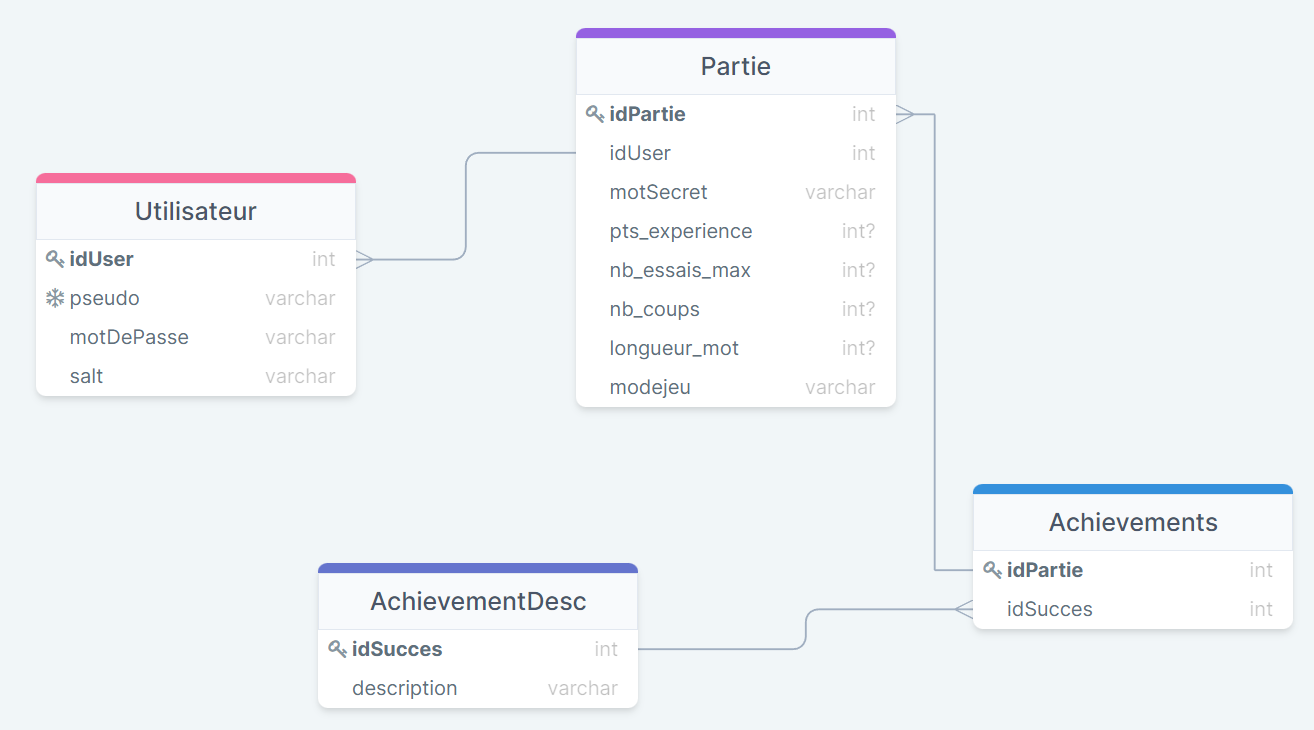
\includegraphics[width=12cm]{figures/bddfinale.PNG}
\caption{Schéma de la base de données de WORDLE}
\end{figure}

\break

\subsubsection{Agencement des pages HTML et des routes}
Le site sera composé de cinq pages HTML :
\begin{itemize}
    \item index.html, la page d’accueil et la page de jeu. Elle est la page centrale du site : depuis index.html, on peut se créer un compte, se connecter et consulter son profil une fois connecté. À noter que créer un compte n’est pas obligatoire pour jouer mais, dans ce cas, aucune partie ne sera enregistrée et aucun achievement ne sera délivré.
    \item register.html, où un joueur peut se créer un compte. Après avoir vérifié que le pseudo renseigné est disponible, les données sont enregistrées dans la table User.
    \item login.html, où le joueur peut se connecter. La connexion réussit si les informations d’authentification (pseudo et mot de passe) renseignées sont valides et échoue sinon.
    \item profile.html, où le joueur peut consulter les informations relatives à son profil. Ces informations sont l’historique des parties effectuées, les statistiques relatives à ces parties et les succès débloqués par le joueur.
    \item settings.html, où le joueur peut choisir le mode de jeu ainsi que la longueur du mot à deviner et le nombre maximum de tentatives autorisées.
\end{itemize}

Quant aux routes, elles seront organisées de la manière suivante :

\begin{figure}[h!]
\centering
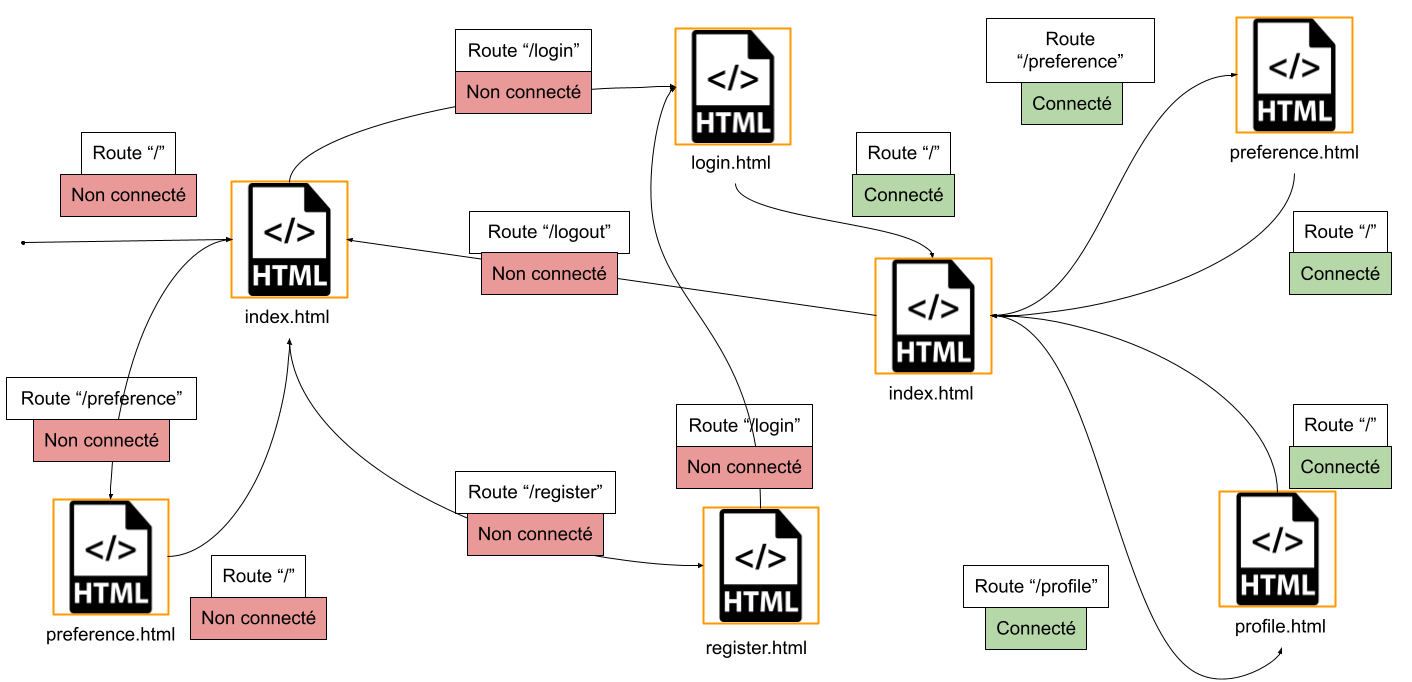
\includegraphics[width=12cm]{figures/schema_routes.png}
\caption{Organisation des routes de WORDLE}
\end{figure}

\subsubsection{Implémentation du jeu}
\textbf{Fonctionnement global} \\

\tabto{1cm}Notre jeu est constitué d’une grille dont les dimensions sont paramétrables par le joueur. Étant donné les paramètres, on crée en JavaScript une grille dont chaque case a un identifiant unique. A l’aide d’un gestionnaire d'événements de clavier, on récupère chaque lettre majuscule tapée par l’utilisateur et on l’insère dans chaque case de la gauche vers la droite jusqu’à ce qu’on atteigne la longueur du mot définie par l’utilisateur. L’utilisateur a également la possibilité d’effacer une lettre rentrée. Aussi, lorsqu’il tape “entrer” et que la longueur du mot entré est égale à celle choisie par l’utilisateur, il verra chaque case contenant chaque lettre se colorer selon la position de la lettre dans le mot secret. Il faut noter que le mot secret est choisi arbitrairement dans le dictionnaire et est caché dans une balise html.\\

\tabto{0cm}\textbf{Fin du jeu}\\

\tabto{1cm}Dans une liste, nous récupérons chaque lettre jusqu’à ce qu’on atteigne la longueur du mot secret. Cette liste est ajoutée dans une autre liste vide définie préalablement et à chaque fois que le mot ne correspond pas au mot secret, on réitère le processus.
Lorsqu’on atteint le nombre d’essais maximum ou lorsque le mot est trouvé, la partie se termine et un bouton “rejouer” s’affiche dans le cas où un utilisateur voudrait rejouer le jeu. 


\subsubsection{Maquette du site}
Voici le premier design du site :

\begin{figure}[h!]
\centering
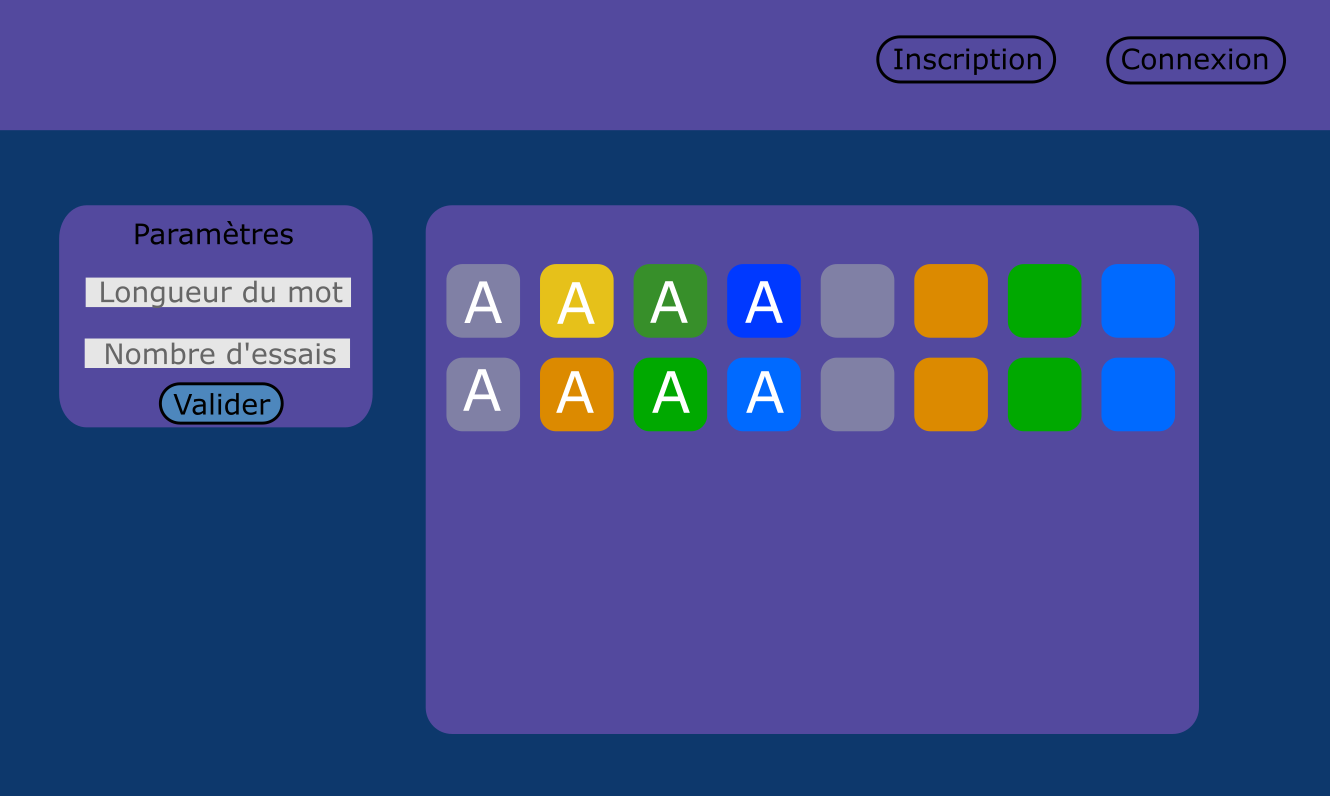
\includegraphics[width=12cm]{figures/wordle_sketch.PNG}
\caption{Première maquette de WORDLE}
\end{figure}
Ce design représente la page index.html lorsque le joueur est déconnecté. Le logo se situerait en haut à gauche. Les couleurs sont potentiellement sujettes à modification.

\subsubsection{Paramétrage du jeu et profil utilisateur}
\tabto{1cm}Le paramétrage du jeu, c’est-à-dire le choix du mode de jeu, de la longueur du mot à deviner ainsi que du nombre de tentatives autorisées est entièrement paramétrable par le joueur sur la page de jeu.

\tabto{1cm}Sur la page profile.html, chaque joueur aura accès à l’historique de ses parties (pour chaque partie, voir quel était le mot secret et si la partie a été gagnée ou non), ses statistiques de jeu (le nombre moyen de coups par partie, le pourcentage de victoire et son nombre de parties jouées) et aux achievements (succès) qu’il aura débloqué en jouant. Pour ce qui est des statistiques, elles seront déclinées en fonction de la longueur du mot : pour chaque longueur de mot différente, on aura un volet “nombre moyen de coups par partie” et un volet “pourcentage de victoire” en plus des statistiques globales.

\subsubsection{Solveur}

\tabto{1cm}Le solveur permet au joueur de penser a un mot que le solveur doit deviner en suivant les règles du jeu. Le solveur est codé exclusivement en langage C et utilise des structures de données les plus appropriées, à savoir une table de hachage permettant au solveur de trouver les mots rapidement. \\

\tabto{1cm}Au lancement du programme, le solveur explique au joueur comment jouer et le joueur répond dans le terminal. Le joueur donne des indices au solveur de la même façon que le jeu WORDLE donne des indices au joueur. Si le joueur veut arrêter le jeu, il met -1 dans le terminal, sinon il donne une chaîne de la même longueur que le mot avec des chiffres 0,1 et 2 : 2 représente une lettre bien placée, 1 représente une lettre correcte mal placée et 0 représente une lettre qui ne se trouve pas dans le mot. En fonction des réponses du joueur, le solveur retourne au joueur le mot le plus probable. Par exemple, si le mot recherché est ARBRE et que le solveur propose NAGER, le joueur est obligé de répondre avec ‘01011’.

\begin{figure}[h!]
\centering
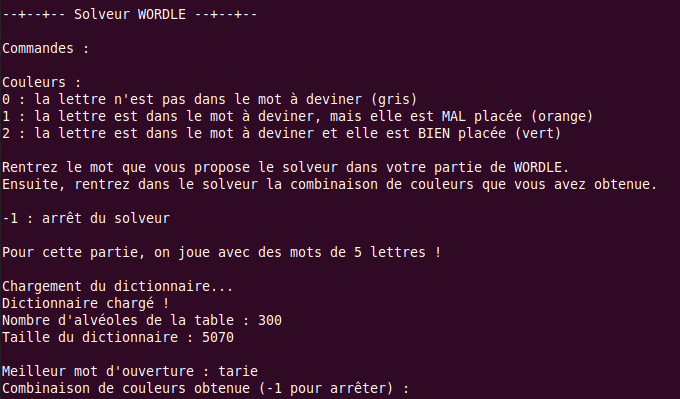
\includegraphics[width=12cm]{figures/avant.PNG}
\caption{Avant de jouer}
\end{figure}

\begin{figure}[h!]
\centering
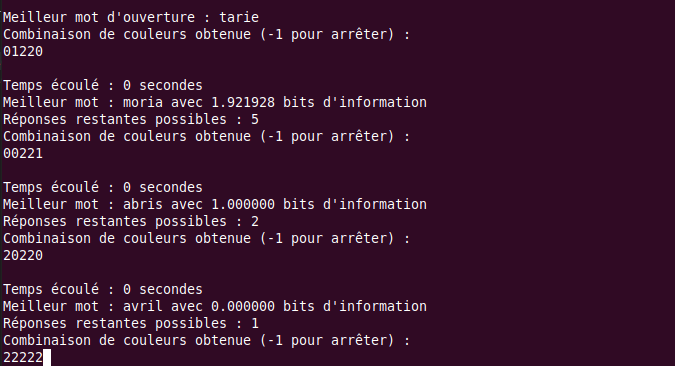
\includegraphics[width=12cm]{figures/solveur_gagne.PNG}
\caption{En jouant}
\end{figure}

\newpage
\section{Bibliographie}

\begin{itemize}
    \item Tutoriel pour jouer à WORDLE (Sean Plays) : https://www.youtube.com/watch?v=PXUqGT5ySsc
    \item Tutoriel sur l’utilisation de la théorie de l’information pour optimiser la résolution d’une session
    WORDLE (3Blue1Brown) : https://www.youtube.com/watch?v=v68zYyaEmEA
    \item Correction d'un bug dans la vidéo précédente (3Blue1Brown) : https://www.youtube.com/watch?v=fRed0Xmc2Wg
    \item Une autre vidéo sur le même sujet (ScienceEtonnante) : https://www.youtube.com/watch?v=iw4\_7ioHWF4
\end{itemize}

\end{document}
